\documentclass[11pt,letterpaper]{article}
\usepackage[T1]{fontenc}
\usepackage[utf8]{inputenc}
\usepackage{lmodern,microtype}
\usepackage[margin=0.85in,headheight=15pt]{geometry}
\usepackage{amsmath,amssymb,amsthm,mathtools}
\usepackage{booktabs,longtable,tabularx,array}
\usepackage{xcolor,graphicx,tikz}
\usetikzlibrary{arrows.meta,positioning,fit,calc}
\usepackage{listings,enumitem,fancyhdr,needspace,xurl}
\usepackage[colorlinks=true,linkcolor=blue!45!black,citecolor=green!35!black,urlcolor=blue!55!black]{hyperref}
\usepackage{bookmark}
\definecolor{ink}{HTML}{183044}
\definecolor{light}{HTML}{F3F6F8}
\definecolor{rule}{HTML}{BDCCD5}
\definecolor{accent}{HTML}{245B78}
\hypersetup{pdftitle={Leant2: Lean-Native, Contract-Directed Program Synthesis},pdfauthor={OpenAI},pdfsubject={Architecture, algorithms, guarantees, and checked prototypes}}
\setlength{\parskip}{4pt}
\setlength{\parindent}{1.1em}
\setlength{\emergencystretch}{3em}
\setlist{itemsep=2pt,topsep=4pt}
\pagestyle{fancy}
\fancyhf{}
\fancyhead[L]{\small\textsc{Leant2}}
\fancyhead[R]{\small Architecture and algorithms}
\fancyfoot[C]{\thepage}
\renewcommand{\headrulewidth}{0.3pt}
\newcommand{\code}[1]{\texttt{\detokenize{#1}}}
\newcommand{\Lean}{Lean~4}
\newcommand{\E}{\mathcal E}
\newcommand{\G}{\mathcal G}
\newcommand{\C}{\mathcal C}
\newcommand{\dom}{\operatorname{dom}}
\newcommand{\supp}{\operatorname{supp}}
\newcommand{\eval}{\operatorname{eval}}
\newcommand{\cost}{\operatorname{cost}}
\newcommand{\unknown}{\mathsf{unknown}}
\newtheorem{theorem}{Theorem}[section]
\newtheorem{proposition}[theorem]{Proposition}
\newtheorem{lemma}[theorem]{Lemma}
\theoremstyle{definition}
\newtheorem{definition}[theorem]{Definition}
\theoremstyle{remark}
\newtheorem{remark}[theorem]{Remark}
\newcolumntype{Y}{>{\raggedright\arraybackslash}X}
\lstdefinelanguage{Lean}{morekeywords={import,open,namespace,end,def,theorem,example,structure,inductive,where,forall,fun,let,in,if,then,else,match,with,by,do,return,partial,unsafe,noncomputable,termination_by,decreasing_by,have,exact,intro,cases,induction,apply,constructor,refine,elab,syntax},sensitive=true,morecomment=[l]{--},morecomment=[s]{/-}{-/},morestring=[b]"}
\lstset{language=Lean,basicstyle=\ttfamily\footnotesize,keywordstyle=\color{accent}\bfseries,commentstyle=\itshape\color{black!55},stringstyle=\color{green!35!black},backgroundcolor=\color{light},frame=single,rulecolor=\color{rule},framesep=5pt,breaklines=true,columns=fullflexible,keepspaces=true,showstringspaces=false,tabsize=2,captionpos=b,aboveskip=8pt,belowskip=7pt,
 literate={α}{{$\alpha$}}1 {β}{{$\beta$}}1 {γ}{{$\gamma$}}1 {→}{{$\to$}}1 {←}{{$\leftarrow$}}1 {∀}{{$\forall$}}1 {×}{{$\times$}}1 {⊕}{{$\oplus$}}1 {⟨}{{$\langle$}}1 {⟩}{{$\rangle$}}1 {·}{{$\cdot$}}1 {∃}{{$\exists$}}1 {¬}{{$\neg$}}1 {≤}{{$\le$}}1 {∧}{{$\land$}}1 {∈}{{$\in$}}1 {≠}{{$\ne$}}1}
\tikzset{box/.style={draw=accent,rounded corners=2pt,fill=light,align=center,inner sep=6pt,font=\small},flow/.style={-{Latex[length=2mm]},thick,draw=accent}}
\begin{document}
\begin{titlepage}
\centering
\vspace*{0.5in}
{\Huge\bfseries\color{ink} Leant2\par}
\vspace{0.18in}
{\LARGE Lean-Native, Contract-Directed\\Program Synthesis\par}
\vspace{0.22in}
{\Large Architecture, Main Algorithms, and\\Kernel-Checked Experimental Foundations\par}
\vspace{0.45in}
{\large September 17, 2026\par}
\vspace{0.35in}
\begin{minipage}{0.91\textwidth}
\textbf{Design objective.} Build a successor to Leant and Djex that treats Lean's actual dependent types, local contexts, universe levels, and behavioral propositions as the synthesis problem itself---not as a richer source language translated into a Haskell-oriented approximation.

\medskip
\textbf{Central recommendation.} Use a typed, contract-carrying obligation graph, with exact Lean expressions as semantic authority; combine focused construction, component composition, recursor-based synthesis, and proof search behind one explicit acceptance boundary.

\medskip
\textbf{Evidence included.} Three small Lean files were compiled remotely in Lean 4.34.0. They exercise native dependent-type search, finite counterexample-guided synthesis, and certified recursive constructions. These are checked foundations, not an implementation of the complete proposed system.
\end{minipage}
\vfill
\begin{tabularx}{\textwidth}{@{}lY@{}}
\toprule
Reviewed Leant revision & \code{6bf05ad78c467989e68290f2d08bbed40802d485}\\
Reviewed Djex revision & \code{e8778f4ebd63e1f9b9b410fa4de8d14a8a04c9e5}\\
Prototype toolchain & Lean 4.34.0; AXLE, through the Wolfram connector\\
Deliverable & Article source and PDF, Lean prototypes, replay tools, and evidence summaries\\
\bottomrule
\end{tabularx}
\end{titlepage}

\begin{abstract}
Leant2 should not be a direct translation of the existing Haskell implementation into Lean. The useful redesign is to make synthesis operate on Lean's own elaborated terms and dependent obligations, while retaining the existing projects' careful separation between proposals, evidence, and acceptance. This article specifies a Lean-only architecture with a native frontend, project-local workers, an exact expression layer, a persistent search-plan layer, and transactional metavariable state. Its core algorithm is focused, bidirectional inhabitant construction over an AND--OR obligation graph. Library composition, dependent case analysis, higher-rank arguments, data-carrying instance dictionaries, and equality transport all use Lean's actual typing operations.

Behavioral constraints are propagated into partial programs, not merely checked after enumeration. Recursive programs are synthesized by choosing eliminators, motives, and algebras; function-valued carriers and generalized recursive hypotheses are first-class search choices. Finite examples, universal propositions, abstract summaries, and external solver suggestions have distinct evidential meanings. Counterexample-guided search and semantic pruning are integrated without confusing finite observation with proof. A single final gate checks the exact program, its exact specification proof, its assumptions, and, when requested, its executability.

The article states conditional soundness and fragment-relative completeness guarantees, gives explicit algorithms and worked traces, proposes implementation modules and acceptance gates, and reports three executable experiments. Native Lean search generated eleven small definitions, including dependent and indexed examples. A finite synthesizer handled all sixteen Boolean functions of two inputs from a 208-candidate grammar and proved their universal correctness. A separate recursive-construction experiment checked a higher-order indexing fold and its specification. These results establish feasibility of selected mechanisms; they do not estimate broad practical coverage.
\end{abstract}

\tableofcontents
\newpage

\section{What Leant2 should be}
\label{sec:thesis}

The primary product should be a \emph{verified implementation synthesizer}, not a theorem prover with a different command name and not a language-model code generator whose output happens to compile. Its input is a Lean type, the current Lean context, optional behavioral constraints, and explicit search policy. Its successful output is an ordinary Lean implementation together with whatever proof the requested mode requires.

Three choices determine the design. First, Lean expressions remain authoritative throughout synthesis. A dependent application such as \code{Vec alpha (n + 1)} must retain its index, not become an opaque surrogate merely because another language's type representation cannot express it. Second, behavioral propositions participate in constructing the implementation. A constraint such as \code{xs = [a]} can solve an output hole; it need not wait until thousands of unrelated lists have been enumerated. Third, synthesis is a portfolio of controlled searches, not one supposedly universal strategy. Composition, structural recursion, index reasoning, and invariant discovery require different methods.

\subsection{The synthesis contract}

Write a request as
\[
 Q=(\E,\Gamma,T,\Phi,X,\G,\Pi,B).
\]
Here $\E$ is the imported declaration environment; $\Gamma$ is the local telescope, including let bindings and instance values; $T$ is the exact target with $\E;\Gamma\vdash T:\mathrm{Sort}\,u$; $\Phi:T\to\mathrm{Prop}$ is an optional hard specification; $X$ is a collection of examples or observations; $\G$ describes allowed construction rules and components; $\Pi$ is a trust and output policy; and $B$ is a vector of resource bounds.

For a specification-bearing success, the essential evidence is
\begin{equation}
 \E;\Gamma\vdash t:T,
 \qquad
 \E;\Gamma\vdash p:\Phi(t).
 \label{eq:success}
\end{equation}
The program and proof need not be packaged in a particular dependent-pair type. Keeping two exact declarations avoids forcing all targets, including proposition-valued or sort-polymorphic ones, through a single data container. A subtype is an excellent user-facing representation when its universe and computational interpretation fit the request, but is not the universal internal representation.

Externally owned metavariables must not be silently solved in a way that changes the question. Preflight either resolves them, freezes them as rigid parameters, or records an explicitly requested elaboration-assistance mode. Only request-owned synthesis holes may be assigned by ordinary search. In particular, assigning an unknown target type to a trivially inhabited type is not a solution to an independently fixed signature.

A type-only request takes $\Phi$ to be the trivial proposition. A request with finitely many example propositions $E_1(t),\ldots,E_k(t)$ can require a proof of their conjunction. This is a theorem about those examples, not a theorem about untested inputs. A universal specification remains universal even when tests are used to accelerate its search.

\subsection{Success is relative to the question actually asked}

The type \code{List Nat -> List Nat} has many useful and useless inhabitants. The type alone does not identify sorting, reversal, filtering, or identity. Even a length-preservation constraint does not distinguish identity from reversal. Leant2 should expose this ambiguity through alternatives and diagnostics, not pretend to infer an unstated intention with logical certainty.

A useful interface offers four closely related products: a term elaborator for filling a typed hole; a tactic for interactive synthesis inside a proof or definition; a command that creates an implementation and named specification theorem; and a batch API used by a project-local worker. A standalone REPL may wrap those same Lean services. There is no Haskell frontend and no requirement to preserve Haskell's interpretation of a signature.

The following is \emph{proposed surface syntax}, not syntax implemented by the accompanying prototypes:
\Needspace{106pt}
\begin{lstlisting}
synth_def lookup : (xs : List alpha) -> Nat -> Option alpha
  satisfying fun f => forall xs i, LookupSpec xs i (f xs i)
  using [List.foldr, Option.some, Option.none]
  config { executable := true, classicalData := false }
\end{lstlisting}
A successful command should create \code{lookup}, \code{lookup_spec}, a machine-readable receipt, and an explanation of the principal construction choices. The source of \code{LookupSpec} is elaborated once under a binder of the exact target type. Unknown names in a specification are errors; they must not silently become new implicit assumptions.

\subsection{The default computational policy}

The default is an executable, total Lean definition. Search procedures themselves may be partial metaprograms, bounded by the host, because their divergence does not make a generated proof valid. Generated programs should not silently use \code{unsafe}, \code{partial}, an unproved termination assumption, or noncomputable selection.

A proof-oriented mode may permit the project's standard classical principles. That does not authorize extracting executable data from arbitrary existential propositions. For example, an assumption \code{Nonempty alpha} or \code{Exists P} is not interchangeable with a computational \code{Inhabited alpha} dictionary or a dependent pair containing a witness. Lean's elimination restrictions must decide which uses are legal. A request that intentionally permits a noncomputable mathematical object should say so and receive a visibly different result category.

\section{Lessons from Leant and Djex}
\label{sec:prior}

The reviewed repositories already contain much more than simple arrow-type enumeration. Their current documentation describes rank-N construction, selected polymorphic instantiation, scoped dictionary evidence, nominal and universe information, typed candidate graphs, and careful replay boundaries. The redesign should preserve those achievements rather than treating the current system as an unsophisticated baseline \cite{leant,djexrank,internals}.

\subsection{The actual boundary to remove}

The reviewed fragment implementation describes a pipeline in which a Lean metaprogram serializes an elaborated expression, and Haskell consumes a synthesis fragment. Structural connectives and some inductive structure are represented explicitly. Term-indexed applications and unsupported dependent structure remain opaque or conservatively restricted. Safety information prevents failed search over that approximation from being promoted to a false noninhabitation claim \cite{fragment}.

The problem is therefore not merely that Haskell syntax is inconvenient. It is that two semantic worlds must continually agree about names, binders, universes, type families, dictionaries, and reconstruction. Leant2 should remove that representational mismatch while preserving the discipline that made the boundary safe.

\begin{table}[ht]
\centering\small
\begin{tabularx}{\textwidth}{@{}p{0.24\textwidth}YY@{}}
\toprule
Concern & Preserve & Change in Leant2\\
\midrule
Type authority & Exact source meaning and scoped evidence & Keep Lean \code{Expr}, levels, local declarations, and eliminator metadata directly.\\
Candidate identity & Evidence belongs to its own candidate & A plan plus its reconstructed expression owns all proofs and observations.\\
Search engines & Focused logic search and ranked typed-hole search & Treat these as cooperating lanes of a dependent obligation engine.\\
Behavior & Positive proof, negative proof, and inconclusive are different & Propagate contracts and counterexamples before a complete term is generated.\\
Negative results & Approximation and bounds cannot establish impossibility & Return actual Lean refutations or explicitly grammar-relative exhaustion.\\
Frontend & Native Lean meaning is authoritative & Remove Haskell compatibility and duplicate source elaboration.\\
\bottomrule
\end{tabularx}
\caption{A semantic redesign, not a loss of existing safety boundaries.}
\end{table}

\subsection{What has already been proposed}

The repository's earlier Lean-rewrite analysis already recommends a Lean controller, a project-local worker, direct expression access, a serializable search representation distinct from metavariable state, and kernel checking of generated candidates. Those are sound architectural foundations, not new claims of this article \cite{rewrite}.

The present design goes further in specifying the synthesis engine: dependent obligation scheduling; contract-to-hole propagation; explicit indexed elimination and transport; recursor and motive discovery; function-valued carrier grammars; proof-aware semantic pruning; and a concrete division between candidate-generation completeness and proof-search completeness. These are the mechanisms needed to make a Lean-native rewrite \emph{more capable}, rather than merely easier to maintain.

\subsection{Behavioral filtering is necessary but not sufficient}

The current named behavioral interface elaborates a proposition about each candidate and attempts checked positive or negative proofs, with bounded decision and simplification methods. Its documentation correctly distinguishes proved examples, proved universal propositions, falsification, and inconclusive checking \cite{behavior}.

Leant2 should retain that final checking behavior but also use the proposition earlier. When synthesizing $f$ under $\forall x,\,f(x)=g(x)$, the equality can constrain the body of $f$. When constructing a dependent record, proof fields can constrain earlier data fields. When synthesizing a recursive step, the global postcondition yields a local induction obligation. Delaying all of that information until complete candidates exist wastes much of the benefit of Lean's type system.

\subsection{Relation to other synthesis and proof-search work}

Refinement-directed synthesis, exemplified by Synquid, motivates interleaving program construction with logical constraints. Type-and-example-directed synthesis motivates propagating observations through partial programs. Type-guided abstraction refinement motivates using abstract component graphs to organize library composition. These methods provide useful algorithmic ingredients; their source-language assumptions and completeness results do not automatically transfer to dependent Lean \cite{synquid,myth,tygar}.

Aesop provides an important model for extensible proof rules, indexing, and controlled proof search \cite{aesop}. It is particularly useful on proposition-valued obligations. It should not simply become the complete program synthesizer: selecting one proof of a fixed proposition can be harmless, while selecting one inhabitant of a data type can determine the program's entire behavior. That distinction will recur throughout the design.

\section{Architecture and ownership}
\label{sec:architecture}

\subsection{One semantic core, several entry points}

The frontend elaborates the target and specification using the project toolchain and imports. It produces an immutable request identity. The worker owns the Lean environment, exact local context, expression cache, and search state. All core synthesis algorithms are written in Lean. External solvers or learned ranking services are optional proposal providers, never required to interpret Lean syntax or certify a result.

\begin{figure}[ht]
\centering
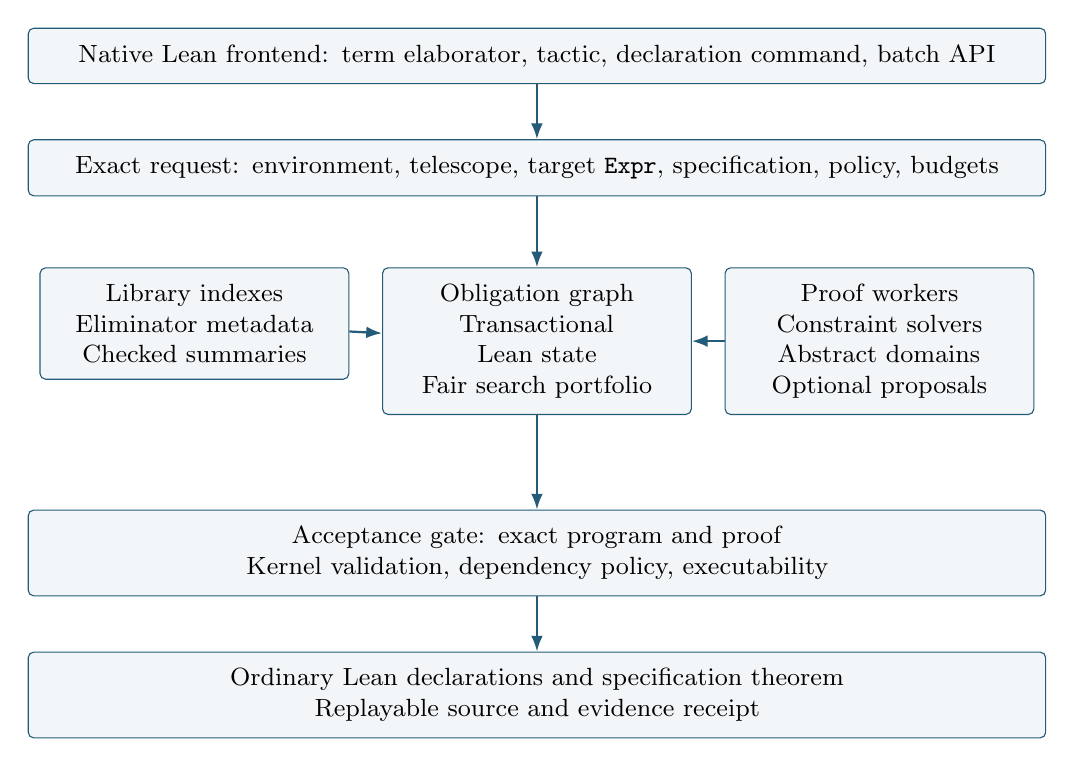
\begin{tikzpicture}[node distance=7mm]
\node[box,text width=12.5cm] (front) {Native Lean frontend: term elaborator, tactic, declaration command, batch API};
\node[box,text width=12.5cm,below=of front] (request) {Exact request: environment, telescope, target \code{Expr}, specification, policy, budgets};
\node[box,text width=3.5cm,below=9mm of request,xshift=-4.35cm] (index) {Library indexes\\Eliminator metadata\\Checked summaries};
\node[box,text width=3.5cm,below=9mm of request] (search) {Obligation graph\\Transactional Lean state\\Fair search portfolio};
\node[box,text width=3.5cm,below=9mm of request,xshift=4.35cm] (constraints) {Proof workers\\Constraint solvers\\Abstract domains\\Optional proposals};
\node[box,text width=12.5cm,below=12mm of search] (gate) {Acceptance gate: exact program and proof\\Kernel validation, dependency policy, executability};
\node[box,text width=12.5cm,below=of gate] (out) {Ordinary Lean declarations and specification theorem\\Replayable source and evidence receipt};
\draw[flow] (front)--(request);
\draw[flow] (request)--(search);
\draw[flow] (index)--(search);
\draw[flow] (constraints)--(search);
\draw[flow] (search)--(gate);
\draw[flow] (gate)--(out);
\end{tikzpicture}
\caption{The proposed data flow. Optional engines can change the order of proposals, but cannot bypass the acceptance gate.}
\end{figure}

The native tactic can run small searches in process for responsiveness. Longer searches should use a replaceable project-local worker. The worker boundary isolates runaway reduction, expensive proof attempts, compiler faults, memory growth, and external evaluation. It also makes the toolchain identity explicit. This is a deployment boundary, not a second language frontend.

\subsection{Three representations, only one type theory}

Leant2 needs three levels of representation, but not three competing definitions of Lean types.

\textbf{Exact semantic objects.} Targets, component types, specifications, and completed terms are Lean expressions with exact universe levels and a known local context. Lean already separates syntax elaboration, expression construction, and kernel checking; Leant2 uses that separation rather than inventing a replacement type checker \cite{leanmanual}.

\textbf{Persistent construction plans.} A plan records lambda introduction, head application, constructor application, case analysis, recursion, sharing, transport, and proof holes. Nodes refer to exact expressions and scope-owned holes. This is a search and provenance representation, not a Haskell-like approximation of types. It can be serialized, costed, replayed, and compared structurally.

\textbf{Ephemeral elaboration state.} A branch carries its own metavariable assignments, local instances, postponed constraints, and elaborator state. These objects must not be shared mutably between sibling alternatives. They are snapshots or replayable transactions owned by one branch.

Raw \code{MVarId} and \code{FVarId} values are not portable identities. To send a task to another process, close expressions over an ordered telescope, encode bound variables by scope-stable positions, preserve levels and constant names, and reopen them with fresh identifiers. An environment fingerprint and protocol version accompany the payload. A worker must reject an expression package whose imports or declaration identities do not match its environment.

\subsection{The request and result lifecycle}

The request identity includes the exact target, specification, local declarations, local-instance ordering, imported environment, enabled rules, and policy. Search runs may have different budgets without changing the mathematical question. A candidate identity additionally includes its plan and exact reconstructed term. A proof or observation is attached to that candidate and question, not to a displayed string.

The result algebra should make unsupported cases and uncertainty visible:
\Needspace{173pt}
\begin{lstlisting}
-- Design sketch: variants, not a compiled interface.
Result :=
  | verifiedProgram term specificationProof receipt
  | verifiedTypeOnly term receipt
  | testedCandidate term observations pendingProofs
  | refutedCandidate term negationProof
  | provedImpossible exactRefutation
  | exhaustedGrammar grammarId explorationCertificate
  | unknown reason residualObligations
  | interrupted resourceState
\end{lstlisting}
A tested candidate is not silently installed as a specification-certified definition. It can be displayed in an explicitly exploratory mode. A command that promises a verified implementation either produces the requested proof or reports that it has not done so.

\subsection{Suggested module boundaries}

\begin{longtable}{@{}p{0.29\textwidth}p{0.66\textwidth}@{}}
\toprule
Lean module family & Responsibility\\
\midrule
\endhead
\code{Leant2.Frontend} & Term, tactic, command, and batch syntax; elaboration of the exact request.\\
\code{Leant2.Core.Request} & Request identity, policy, budget vector, result categories, immutable specification.\\
\code{Leant2.Core.Plan} & Scoped plan DAG, hole dependencies, costs, and provenance.\\
\code{Leant2.Meta.Scope} & Telescope closing and reopening, universe freshness, context snapshots.\\
\code{Leant2.Meta.Refine} & Exact Lean application, introduction, constructor, equality, and elimination operations.\\
\code{Leant2.Search} & Resumable cursors, queues, iterative deepening, lane fairness, and accounting.\\
\code{Leant2.Index} & Local and global component retrieval, discriminators, signatures, recursor metadata.\\
\code{Leant2.Contract} & Proposition elaboration, path conditions, dependency propagation, and proof obligations.\\
\code{Leant2.Recursion} & Structural schemas, motives, carriers, recursive-call capabilities, and well-founded templates.\\
\code{Leant2.Semantics} & Typed observations, counterexamples, checked summaries, and abstract-domain plugins.\\
\code{Leant2.Proof} & Bounded proof portfolios and proof-producing arithmetic or rewriting adapters.\\
\code{Leant2.Check} & Closed declaration validation, axiom and dependency audit, executability checks.\\
\code{Leant2.Export} & Source presentation, exact re-elaboration, receipts, and independent-replay bundles.\\
\code{Leant2.Worker} & Project-toolchain process lifecycle, protocol, cancellation, and resource isolation.\\
\bottomrule
\end{longtable}

Keep the core package dependent only on Lean and its standard libraries. Put Mathlib-dependent proof methods, SMT adapters, and learned ranking in optional packages. That allows ordinary Lean projects to use type-directed synthesis without importing a large mathematics library, while richer projects can exploit their existing proof infrastructure.

\section{The dependent obligation graph}
\label{sec:graph}

\subsection{Why a tree of independent typed holes is insufficient}

Consider a target $\Sigma n:\mathbb N,\,\mathrm{Vec}\,\alpha\,n$. Choosing the first field changes the type of the second. Conversely, discovering that a available vector has length $k$ can determine the first field. A record's proof field may constrain its data fields. Two arguments of one component may share a type metavariable or a dictionary selection. Independent recursive calls to ``synthesize this type'' lose these correlations.

The state must therefore be a graph of \emph{coupled obligations}. It is an AND--OR graph: applying a component creates several jointly required children; choosing a different component creates an alternative branch. Shared metavariables and specification dependencies create edges beyond the parent--child tree.

A hole record should contain at least
\[
 H=(\mathrm{id},\Gamma_H,T_H,\Phi_H,D_H,R_H,O_H,s_H),
\]
where $D_H$ is a dependency set, $R_H$ is the available recursive-call capability set, $O_H$ contains typed observations, and $s_H$ is a scope and assignment generation. The exact expressions $T_H$ and $\Phi_H$ may contain branch-owned metavariables. Every occurrence records which assignments can invalidate cached facts about it.

\subsection{Four invariants}

\begin{enumerate}
\item \textbf{Scope closure.} Every free variable in a hole's type, contract, observations, or proposed solution is in its allowed telescope. Substitution may not introduce a younger local into an older scope.
\item \textbf{Type coherence.} Each refined plan reconstructs, under its branch state, to a term of the recorded type. An unresolved proof obligation remains an obligation rather than an assumed fact.
\item \textbf{Dependency coherence.} Changing a metavariable invalidates all observations and indexes whose recorded support depends on it. Unrelated subproblems may remain reusable.
\item \textbf{Evidence ownership.} A proof, counterexample, semantic summary, or cost theorem is meaningful only for its exact expression, context, specification, and policy.
\end{enumerate}

These invariants are more important than the precise choice of priority queue. Violating them can turn a plausible implementation into a proof of a different statement, or can make a supposedly harmless cache delete the only viable candidate.

\subsection{Transaction boundaries}

Every speculative refinement starts from a saved elaboration state. The refinement can introduce metavariables, solve equalities, select an instance, split a context, and create child goals. A successful continuation commits the complete resulting state. Failure restores the saved state, including assignments made by unification before the failure occurred.

The native prototype uses \code{Tactic.saveState} and restoration around each alternative. A production implementation should wrap the relevant Lean version's APIs behind a narrow adapter. It must distinguish ordinary rule failure from interrupts, exhausted heartbeats, and corrupted worker state. Catching every exception as ``this rule is inapplicable'' is acceptable only as a small experimental simplification, not as the system's lifecycle policy.

\Needspace{240pt}
\begin{lstlisting}[caption={Transactional refinement over coupled obligations. Pseudocode.}]
refineBranch(branch, rule):
  snapshot := saveFullElaborationState()
  try:
    restore(branch.state)
    proposal := rule(branch.focus)
    checkScopeAndDependencies(proposal)
    propagateSolvedAssignments(proposal)
    children := classifyResidualObligations(proposal)
    next := branch.with(proposal.plan, children, saveState())
    return Success(next)
  catch OrdinaryInapplicability:
    return Inapplicable
  catch ResourceInterrupt as reason:
    return Suspended(branch, reason)
  finally:
    restore(snapshot)
\end{lstlisting}

The pseudocode restores the caller's state even when it returns a successful child: the child owns the saved successor state. In a depth-first implementation, a successful branch may instead remain installed until the caller commits or backtracks. Mixing these two conventions is a common source of stale assignments; choose one explicitly.

\subsection{Scheduling dependent children}

A simple left-to-right field order is predictable, but often inefficient. A better scheduler chooses a ready obligation with high expected information gain: a rigid equality that may determine a data hole; a constructor field with a small finite type; or a proof obligation whose simplification exposes an impossible branch. An obligation is ready when the variables needed by the chosen rule are sufficiently instantiated, not necessarily when every metavariable in its type has disappeared.

Maintain a worklist of delayed equalities and class obligations. An assignment wakes only the obligations that mention its support. For a strongly connected group, solve or branch over the group as a unit. Do not diagnose cyclic dependencies as logical inconsistency: they may simply require choosing a constructor or a polymorphic instantiation first.

\section{Lean-native elaboration and matching}
\label{sec:matching}

\subsection{Binders, universes, and local instances}

Introduce a dependent function by opening its exact binder. Preserve explicit, implicit, strict-implicit, and instance-implicit binder information in the plan and exported source. The fresh local is rigid with respect to earlier holes. A component application gets fresh metavariables for its own implicit arguments and fresh universe metavariables for that occurrence, not globally shared choices.

Lean's \code{Prop} is impredicative, whereas its data universe hierarchy is predicative and non-cumulative. Retaining a polymorphic argument therefore does not license arbitrary Haskell-style impredicative data instantiation. Level constraints and the actual elaborated type decide whether an application is legal \cite{leanmanual}. A search bound on proposed instantiations is an operational limitation; it is not a new rule restricting Lean to some fixed rank.

Typeclass synthesis is a component of elaboration, not an alternative definition of semantics. Local dictionaries can carry different data. Two values of the same \code{Inhabited Nat} type can provide different defaults; two algebra dictionaries can provide different operations. The selected dictionary expression and local-instance context are part of candidate identity. Proof irrelevance does not identify these data values.

\subsection{Definitional equality is an operation, not a global canonicalizer}

Use bounded weak-head normalization to reveal a function, constructor family, or reducible alias. Use Lean's definitional-equality machinery transactionally to match a component's result against the target. An unsuccessful or interrupted matching attempt is not a theorem that the types are unequal. It may reflect unresolved variables, transparency settings, or a resource limit.

Do not promise a canonical normal form for arbitrary Lean expressions. Do not key all caches by pretty-printed normal forms. Store exact expressions, the normalization policy, and the assignments on which the result depended. Lean's implementation and metatheory contain subtleties that make a blanket assumption of a terminating, globally canonical conversion procedure inappropriate \cite{leanmanual}.

When equality is only propositional, create an explicit transport obligation. A candidate of type \code{Vec alpha (n + 0)} may be definitionally compatible with one target under a particular reduction orientation, while a more complicated index equality may require a theorem and a cast. The search should try inexpensive definitional matching first, then registered proof-producing index normalizers, and finally a bounded general equality proof. None of these may silently change the requested type.

\subsection{Head-spine application}

For a local or global component $h$ with type
\[
 \Pi x_1:A_1.\,\Pi x_2:A_2(x_1).\cdots\Pi x_k:A_k(\vec x_{<k}).\,R(\vec x),
\]
application search creates fresh argument holes, forms the tentative expression $h\,?x_1\cdots?x_k$, and matches $R(\vec{?x})$ against the requested result. It then solves the remaining argument, universe, instance, and proof obligations in their dependency graph.

It must also consider \emph{prefixes} of this spine. A function may itself be the desired value, or a partially applied function may be the correct higher-order argument. Fully saturating every provider before checking its type misses ordinary compositions. Conversely, blindly enumerating all implicit arguments before result matching creates an unnecessary Cartesian product. Result-directed unification should determine correlated choices first.

\Needspace{162pt}
\begin{lstlisting}[caption={Demand-directed component application. Pseudocode.}]
applyHead(goal, head):
  for prefix in resumableApplicationPrefixes(head.type):
    transaction:
      freshenUniverseParameters(head)
      arguments := openDependentSpine(prefix)
      expression := apply(head, arguments)
      matchResult(expression.type, goal.type)
      propagate(goal.contract, expression)
      emit(expression, unresolved(arguments), delayedConstraints)
\end{lstlisting}

The prefix iterator is itself bounded and resumable. Repeated uses of the same head are allowed. A ban on repeated head use can exclude $f(f(x))$, a required fold composition, or a useful recursive algebra. Such restrictions belong only in an explicitly heuristic lane, with an unrestricted baseline available when its grammar is enabled.

\subsection{Higher-rank arguments and scoped instantiation}

Suppose a component expects $(\Pi\alpha:\mathrm{Type},\alpha\to\alpha)\to\mathbb N$. Synthesis of its argument opens a fresh type variable and value, then constructs the body under that private scope. The variable cannot escape into a metavariable created outside the scope. Direct forwarding of an available polymorphic value should be tried before reconstructing an eta-expanded equivalent.

Unsolved type-level choices can draw from a growing, typed vocabulary: rigid type variables in scope; exact type subexpressions in the request; types exposed by retrieved components; and explicitly enabled type constructors applied to smaller choices. This is a search grammar over Lean expressions, not a replacement kind system. General higher-order unification is not assumed. Stuck higher-order constraints are suspended or explored through bounded instantiations; failure remains inconclusive.

\section{The core construction algorithm}
\label{sec:core}

\subsection{Focused construction rules}

The core should combine checking against an expected type with synthesis of neutral applications. Its principal rules are:

\textbf{Introduction.} Open a dependent function binder, construct a record or inductive constructor, or build a dependent pair. Constructor arguments are not assumed independent. The result index is unified with the target before impossible alternatives are pursued.

\textbf{Forwarding and application.} Use an exact local value, a compatible partially applied head, or a retrieved component. Both computational and proposition-valued arguments enter the same dependency graph, but may be solved by different engines.

\textbf{Elimination.} Split an available inductive value using Lean's actual eliminator and an inferred or synthesized motive. Refine indices and the dependent local context in every branch. Use equality elimination and no-confusion principles to discharge impossible branches.

\textbf{Proof closure.} Close propositions by assumption, reflexivity, simplification, registered decision procedures, or a bounded proof portfolio. A proof rule may solve shared computational metavariables; those assignments must be checked and recorded just like assignments made by a program-construction rule.

\textbf{Recursion and sharing.} Introduce an approved recursor schema or a let-bound helper when simpler rules are insufficient. These are controlled search expansions, not unrestricted self-reference.

\subsection{What focusing can and cannot safely discard}

For a fixed proposition, there is usually no need to enumerate many proof terms merely because they are syntactically different. For a data target, however, different constructors or arguments can produce different behavior. Even eta expansion, while logically benign in suitable cases, can affect the size and shape of later search.

Accordingly, define \emph{proof normalization} separately from \emph{program alternatives}. A rule may be called safe for the proof lane when it preserves solvability of the fixed proposition. It is not automatically safe for discarding inhabitants of an enclosing data hole. For example, selecting zero for a natural-number hole is type-correct, but may prevent a later proof of a dependent property that requires one.

\subsection{Dependent elimination}

For a local $x:I(\vec p,\vec i)$, the motive must account for the goal's dependence on $x$, on its indices, and on other local declarations that depend on it. The implementation should use the appropriate Lean elimination operations and metadata rather than reimplementing dependent pattern matching by replacing strings or constructor names.

An impossible constructor branch is removed only after an exact unification contradiction or a checked contradiction proof. For an indexed vector of length $n+1$, the nil case is not discarded because the name ``nil'' looks inappropriate: the eliminator generates the relevant index equalities and the branch is discharged from them. The native experiment's printed vector-head term illustrates this process through equality and heterogeneous-equality transport.

Elimination from propositions requires particular care. An existential proof does not generally authorize construction of arbitrary data by pattern matching. Equality and empty propositions have special eliminators, and some singleton propositions admit broader elimination. Query Lean's actual recursor information and let the final checker enforce the restrictions; do not install a blanket rule ``every inductive can be case-split into every sort.''

\subsection{A baseline search with a precise scope}

Keep a simple, deterministic iterative-deepening lane over a declared construction grammar. Its cost may count constructor and application nodes, case splits, recursion schemas, and argument instantiations. Each finite layer is explored with explicit accounting. This lane is valuable as a regression baseline and as a completeness-preserving alternative to aggressively ranked search.

A production engine need not run the baseline exclusively. It can devote most work to contract-guided and component-guided lanes, while reserving a fixed fraction for baseline progress. A completeness statement is meaningful only for the enabled grammar, its instantiation vocabulary, its elimination and recursion schemas, and the proof procedures assumed complete. Merely using Lean's actual types does not make the search complete for all Lean inhabitants.

\Needspace{206pt}
\begin{lstlisting}[caption={Portfolio-level synthesis loop. Pseudocode.}]
run(request):
  lanes := initializeEnabledLanes(request)
  while budgetRemains():
    lane := fairRunnableLane(lanes)
    event := lane.advance(oneChargedQuantum)
    match event:
      | partialPlan p => propagateAndEnqueue(p)
      | completeTerm t => scheduleExactVerification(t)
      | checkedCounterexample c => updateOwnedExampleBank(c)
      | verified t proof => return acceptanceGate(t, proof)
      | suspended s => retainContinuation(s)
      | finished evidence => recordLaneScope(evidence)
  return summarizeUnknownAndExhaustedFragments()
\end{lstlisting}

The important scheduling unit is charged work, not ``one next candidate.'' A supposedly lazy stream can spend an unbounded amount of time producing its next element. Every expensive iterator---component retrieval, instantiation, recursive schema generation, and proof checking---must expose suspension points or run under an isolatable bound.

\section{Library-guided composition}
\label{sec:library}

\subsection{Retrieval is part of the algorithm}

Practical Lean types often become easy once the correct constructor, projection, theorem, or library combinator is available. Searching every imported declaration at every hole is expensive; retrieving only exact textual matches is incomplete even for elementary composition. Leant2 therefore needs a typed retrieval layer, not merely a list of globally enabled constants.

Index declarations by weak-head-normalized result head, visible and implicit arity, argument head symbols, universe parameters, binder dependencies, and a coarse classification of computational versus proof arguments. Keep wildcard buckets for results that remain flexible. Record projections and constructor families explicitly. For a type alias, preserve both its nominal identity and the reduction policy used to expose its head.

A query should search in a growing sequence: exact locals and selected dictionaries; constructors and projections directly associated with the goal; explicitly registered project components; nearby imported declarations; and broader library slices. These are preference tiers, not assertions that useful terms cannot occur outside a tier. A fair broadening lane prevents the early retrieval cutoff from becoming an invisible language restriction.

\subsection{Backward demand and forward availability}

Backward search asks what component can produce the desired result. Forward search asks which useful intermediate values can be built from what is already available. Either alone can be inefficient. Combine them in a demand graph: each result type is a demand node; a component application creates a hyperedge from its argument demands to its result; available locals seed solved demands.

In the dependent setting, nodes are not simply types modulo an informal equality. A node also has a telescope, outstanding assignments, selected instances, and a scope. Two occurrences with different vector lengths or dictionary payloads must remain distinct unless an exact transport or equivalence justifies their identification.

A practical optimization is to maintain coarse abstract nodes for retrieval and exact scoped obligations for validation. The abstract graph can suggest a short chain of components. Reconstruct that chain with real Lean expressions; if exact matching fails, refine the abstract distinction that caused the false positive. This borrows the organizational idea of type-guided abstraction refinement without assuming that an abstraction of dependent Lean types is complete \cite{tygar}.

\subsection{Component summaries}

A component entry may include checked theorems describing its behavior. For a function $c:A\to B$, a useful summary has the form
\[
 \forall x,\quad P(x)\to R(x,c(x)).
\]
For a higher-order component, the summary can quantify over callback behavior. A fold summary can state preservation of an invariant, while a map summary can relate output length and element properties to its input and callback.

Summaries should be elaborated Lean declarations with explicit parameters, not untrusted strings interpreted as facts. Instantiate them in the same branch and with the same dictionary and universe choices as the component itself. A summary about one instance of an overloaded operation does not authorize another instance. If a summary is unavailable, the component remains usable; only the optimization is lost.

The summary index should include theorem direction and intended use: backward obligation generation, forward fact propagation, or proof closure. A theorem can be logically correct but operationally disastrous when repeatedly oriented in the wrong direction. Register a cost, preconditions, and an unfolding policy, and charge unsuccessful instantiations.

\subsection{Avoiding accidental oracle synthesis}

For ordinary use, returning an already available function that meets the specification is a success, often the best one. For evaluating synthesis ability, however, a hidden reference implementation must not become a component merely because it occurs in the specification's source file.

The benchmark harness should whitelist component declarations and inspect the generated program's computational dependencies. Specification and proof dependencies must be distinguished from runtime dependencies: a theorem about equality to a reference function naturally mentions that reference, but the synthesized program should not call it when the task is meant to test invention. Report direct reuse, composition, and newly constructed recursion separately. A large pass count consisting mainly of reference retrieval is not evidence for recursive synthesis.

\section{Recursion as motive and algebra synthesis}
\label{sec:recursion}

Recursion is the principal difference between synthesizing type-correct plumbing and synthesizing many useful programs. The recommended approach is not to introduce an unconstrained recursive function symbol and hope to prove termination later. Instead, select an approved recursive schema whose legal recursive calls are explicit, then synthesize its motive and branch algebra.

Lean elaborates structural and well-founded recursive definitions into logical constructions with precise obligations. Its kernel does not independently run the surface termination checker; the elaborated term must justify the definition through accepted primitives and recursors \cite{leanrec}. Leant2 should exploit that infrastructure while preserving a separately tested route to executable code.

\subsection{The recursion ladder}

Use increasingly general constructions in a visible order. First try existing library combinators with appropriate summaries: \code{map}, \code{foldr}, \code{foldl}, option combinators, traversals, and registered domain-specific recursors. Next synthesize a structurally recursive definition over an input inductive. Then try generalized accumulators, function-valued carriers, and paired results. Finally enable well-founded or lexicographic recursion with explicit decreasing-call obligations.

This ordering is a heuristic, not a theorem that folds are always sufficient or efficient. In particular, nested and indexed inductives may require a recursor whose motive depends on several indices and local values. The search registry should expose what each schema supports and what remains outside its scope.

\subsection{A certified motive}

Suppose the desired implementation has input $x:I$ and output $y:B(x)$ with specification $R(x,y)$. A powerful schema constructs a value in
\begin{equation}
 M(x)=\{y:B(x)\mid R(x,y)\}.
 \label{eq:certifiedmotive}
\end{equation}
For each constructor of $I$, the branch receives its ordinary fields and certified recursive results for its recursive fields. The branch must construct a new output and prove its local postcondition. Projection then yields the requested implementation; the proof projection yields its specification.

This is not a claim that subtype packaging is always the most efficient internal term. The equivalent implementation can synthesize the program and induction proof separately, sharing the same plan. The conceptual benefit is that the correct induction hypothesis is derived from the motive, rather than guessed independently after the program has been generated.

For lists, a standard summary is
\begin{align*}
 &R([],z),\\
 &\forall x,xs,v,\quad R(xs,v)\to R(x::xs,s(x,v))\\
 &\hspace{3em}\Longrightarrow\quad
 \forall xs,\ R(xs,\mathrm{foldr}\ s\ z\ xs).
\end{align*}
The accompanying \code{fold_contract} theorem proves this statement in Lean. A more general list recursor branch can also receive $xs$ itself, not just its recursive result. That is important when the output or proof depends on the original tail.

\subsection{Recursive-call capabilities}

Represent each allowed recursive call as a capability with an exact argument telescope and a smaller-than justification. In a structural list branch, the capability supplies the result for the particular tail. In an indexed recursor, it supplies a result at the tail's refined index. In a well-founded schema, it has the form
\[
 \mathrm{rec} : \Pi y,\ R_{\mathrm{dec}}(y,x)\to B(y).
\]
If constructing certified outputs, replace $B(y)$ by the certified motive. A candidate can call this capability only by supplying the required argument and decrease proof. It cannot call an unrestricted version of itself on the current input.

This makes termination constraints local. It also improves synthesis: an attempted recursive call immediately reveals which measure fact is missing. The missing fact becomes a proof obligation rather than a later, opaque rejection of an otherwise large candidate.

\subsection{Carrier synthesis must include functions}

A fold's carrier is the type of its accumulated result. Restricting carriers to the final scalar output type misses many useful programs. An index lookup can be represented by a fold whose result is itself a function:
\[
 C = \mathbb N\to\mathrm{Option}\,\alpha.
\]
The base and step are
\begin{align}
 z(i)&=\mathrm{none},\nonumber\\
 s(x,r)(0)&=\mathrm{some}(x),\label{eq:indexstep}\\
 s(x,r)(k+1)&=r(k).\nonumber
\end{align}
Then $\mathrm{foldr}\ s\ z\ xs$ is a lookup function for the list. The future index is handled \emph{inside} the fold result. There is no need to force a fixed index to travel as an unrelated external parameter during every composition choice.

The checked \code{indexFold} experiment uses exactly this carrier and proves equality to an independently written structural specification for every list and natural index. The carrier and algebra were supplied by hand in that experiment; discovering them autonomously is an architectural objective, not a measured accomplishment.

The carrier generator should use a bounded grammar seeded by types already demanded by the goal and its components:
\[
 C ::= A \mid C_1\times C_2 \mid \mathrm{Option}\,C
       \mid D\to C \mid \Sigma d:D,\,C(d),
\]
where $A$ and $D$ range over a typed, scope-valid vocabulary. Enable dependent carriers only when their elaboration succeeds and the chosen schema supports them. Grow grammar size fairly. A fixed finite initial vocabulary is an optimization tier, not a universal completeness claim.

A useful demand rule is \emph{parameter postponement}: when a recursive program receives an input $xs$ and a later parameter $q$, propose a carrier $\mathrm{type}(q)\to B$ before enumerating arbitrary auxiliary types. A second rule is \emph{result pairing}: when a recursive step needs a property or auxiliary value of its recursive result, propose a paired carrier containing that value. A third is \emph{accumulator generalization}: move a changing parameter into an explicit generalized recursive hypothesis.

\subsection{Worked trace: discovering the indexing algebra}

Assume the request is $\mathrm{List}\,\alpha\to\mathbb N\to\mathrm{Option}\,\alpha$, with a relational lookup specification. Component retrieval finds a right fold. Parameter postponement proposes $C=\mathbb N\to\mathrm{Option}\,\alpha$. The fold generates the base obligation
\[
 z:\mathbb N\to\mathrm{Option}\,\alpha
\]
and the step obligation
\[
 s:\alpha\to C\to C.
\]
The empty-list specification requires $z(i)=\mathrm{none}$ for all $i$, so constructor-directed proof propagation produces the constant-none base.

For the step, introduce $x:\alpha$, $r:C$, and $i:\mathbb N$. Case analysis on $i$ creates the zero and successor branches. The zero specification requires the result to be $\mathrm{some}(x)$. In the successor branch, the recursive hypothesis says that $r(k)$ implements lookup in the tail at $k$. The desired postcondition for the cons list reduces to that hypothesis. The resulting algebra is exactly Equation~\eqref{eq:indexstep}.

A complete implementation of this trace requires a registered relationship between the lookup specification's cons/successor clause and its tail clause, or a proof procedure capable of exposing that relationship. The algorithm does not learn it merely from the word ``lookup.'' When the required lemma is absent or too expensive to prove, the residual proof obligation should be reported.

\subsection{Dependent lookup and impossible branches}

For a length-indexed vector, consider
\[
 \Pi n:\mathbb N,\quad \mathrm{Vec}\,\alpha\,n\to\mathrm{Fin}\,n\to\alpha.
\]
A suitable motive for elimination on the vector is
\[
 M(n,xs)=\mathrm{Fin}\,n\to\alpha.
\]
The nil branch receives an index in \code{Fin 0}, which is eliminated through its impossible bound. The cons branch inspects the finite index: zero returns the head; a successor index supplies a smaller finite index for the recursive result. Index arithmetic and conversions are proof obligations, not erased annotations.

The motive grammar should derive this shape by abstracting the vector's index and retaining later arguments in the result. It should not guess a nondependent result $\alpha$ and then try to repair missing index information afterward. The simpler vector-head prototype validates indexed elimination, but does not implement this full lookup synthesis trace.

\subsection{Reversal and auxiliary state}

For reversal, a naive right-fold algebra may need append and produce quadratic behavior. A difference-list carrier $\mathrm{List}\,\alpha\to\mathrm{List}\,\alpha$ or an explicitly generalized accumulator gives a different search space. A useful invariant can describe the accumulated function by
\[
 \forall ys,\quad d(ys)=\mathrm{reverse}(xs)\mathbin{++}ys.
\]
A candidate algebra must prove the base and step equations for this invariant. Alternatively, a left-fold schema can expose an accumulator directly. The search should retain multiple certified implementations and rank them using an explicit cost model, rather than calling the shortest proof or smallest syntax tree ``fastest.''

This example illustrates why invariant templates and carrier choices should be coupled. Choosing a function carrier without a specification relating its future argument to the intended output leaves an enormous unconstrained higher-order space. Conversely, the generalized invariant almost determines the useful carrier.

\subsection{Well-founded and mutual recursion}

When structural schemas fail, enable a well-founded lane. Its first measure candidates should be supplied measures, structural sizes, natural arguments, and lexicographic tuples of those quantities. Each proposed call generates a decrease goal. Arithmetic methods may discharge simple goals, while registered domain lemmas handle more semantic decreases.

A well-founded template is not allowed to turn an unproved decrease into an axiom, nor may it silently replace the requested algorithm by a fuelled partial approximation. A fuelled implementation is valid only when fuel is part of the requested interface or a theorem proves sufficient fuel for every permitted input.

Mutual recursion can be represented by a tagged domain with a shared well-founded relation, or by a registered mutual recursor whose branches and recursive results are explicit. Nested inductives require their actual recursor structure and, often, map-like recursive results over nested fields. These should be supported incrementally through metadata-driven schemas; treating every nested field as an ordinary immediate subterm is unsound.

\subsection{Logical reconstruction and executable lowering}

A mathematical recursor expression can be kernel-accepted yet unsupported by a particular code-generation path. The initial recursive prototype exposed exactly this issue: a bare \code{List.rec} definition passed logical axiom inspection but produced a code-generator error. Rewriting the same certified construction using structural equations compiled successfully.

Consequently, recursion plans need two coordinated products: a logical reconstruction and an executable definition schema. Prefer Lean's equation compiler for newly synthesized recursive declarations, retaining the exact branch plans and termination evidence. If an alternative executable lowering is used, prove its correspondence to the logical candidate and check both declarations. A request for an executable implementation is not complete merely because its mathematical expression has a type.

\section{Behavioral constraints as active obligations}
\label{sec:contracts}

\subsection{A hierarchy of specification languages, not a hierarchy of truth}

The exact hard specification is always a Lean proposition. Specialized plugins may recognize useful fragments: finite equalities, arithmetic relations, list lengths, membership, permutations, relational postconditions, or component-specific invariants. Recognition determines available algorithms; it does not replace the proposition by a weaker one.

A recognized fragment can carry a proof-producing translation. An unrecognized fragment remains an ordinary Lean proof obligation. This fallback is essential for broad practical coverage: many requests mix an easily recognized computational structure with one unusual lemma. Refusing the entire type because one proposition lies outside an SMT fragment would recreate the limitations of a restrictive source translation.

\subsection{Propagation through program structure}

Constraint propagation should be rule-specific and justified. For a lambda, a pointwise specification creates a body obligation under the new argument. For a constructor, projection equations and registered constructor lemmas relate the output contract to its fields. For a conditional on a decidable proposition $P$, each branch receives its corresponding path assumption. For an application, a checked component summary can turn the desired postcondition into preconditions on arguments and callbacks.

The engine need not synthesize a globally minimal weakest precondition for every Lean term. That is unrealistic. Instead, it should apply a finite collection of useful, checked implication rules. If $W$ is a proposed sufficient condition and the plugin supplies
\[
 W\to\Phi(t),
\]
then solving $W$ is a sound route to the target. Failure to solve $W$ is not a proof that $\Phi(t)$ is false, because $W$ need not be necessary.

\subsection{Proof holes can determine data holes}

Consider
\Needspace{83pt}
\begin{lstlisting}
def singleton (a : alpha) : {xs : List alpha // xs = [a]} := by
  leant2_core []
\end{lstlisting}
The subtype constructor produces a data metavariable $?xs$ and a proof obligation $?xs=[a]$. Reflexivity and unification can solve the data metavariable by $[a]$. This is legitimate joint synthesis: the property restricts the witness, and the final constructor checks the witness and its proof together.

The same effect appears with dependent pairs, lengths, and equations between component results. A production scheduler should exploit it deliberately. It should not force every data hole to be independently enumerated before any proof hole is examined. At the same time, assignments made by proof search must obey the original executable and dependency policy; a proof tactic may not introduce an unacceptable noncomputable implementation and hide it behind a successful theorem.

\subsection{Typed examples for dependent functions}

For a dependent function $f:\Pi x:A,B(x)$, an input observation has an input $a:A$ and an output expectation in the exact fiber $B(a)$. For a telescope of inputs, later inputs may depend on earlier ones and may include validity proofs. Store examples as elaborated terms with those dependencies, not as loosely typed JSON tuples.

Equality-based examples are one possibility, but relational observations are often better. A sorting example may require the output to be sorted and a permutation of the input, rather than selecting one particular representation. A nondeterministic relation can admit multiple correct outputs. An effectful computation needs an explicitly chosen semantics for traces, state, or observations; directly running arbitrary \code{IO} during search is neither a proof nor a safe default.

\subsection{Universal and relational specifications}

A universal proposition need not have an executable decider. Leant2 should try proof-producing simplification, induction, arithmetic, and component summaries without pretending that a finite test run decides it. When a property relates two executions, such as equivariance, noninterference, or a homomorphism law, a collection of independent single-run examples can miss the relation entirely. Store the relational structure and use paired or symbolic executions only through an appropriate plugin.

A useful extension interface distinguishes three outputs from a contract analysis:
\Needspace{106pt}
\begin{lstlisting}
ContractAnalysis :=
  | sufficientObligations subgoals implicationProofBuilder
  | necessaryConstraint constraint necessityProof
  | heuristicHint hint
\end{lstlisting}
A sufficient condition guides construction. A necessary condition can justify excluding a branch when its impossibility is certified. A heuristic hint changes priority only. Conflating these categories is one of the easiest ways to lose valid programs while believing the search remains complete.

\section{Counterexample-guided synthesis}
\label{sec:cegis}

\subsection{The exact loop}

Counterexample-guided inductive synthesis, or CEGIS, alternates between finding a candidate consistent with current observations and verifying it against the full specification. Let $X_k$ be the current example bank. The construction engine proposes $t_k$ satisfying the constraints induced by $X_k$. Verification then has three semantic outcomes:
\[
 \mathsf{Proved}(p:\Phi(t_k)),\qquad
 \mathsf{Refuted}(q:\neg\Phi(t_k)),\qquad
 \mathsf{Unknown}.
\]
When the negation has an executable witness shape, a concrete counterexample can be extracted or reconstructed and replayed. Otherwise, a proof of $\neg\Phi(t_k)$ still rejects that candidate, but does not automatically yield a useful input example for other candidates.

\Needspace{262pt}
\begin{lstlisting}[caption={Proof-aware CEGIS. Pseudocode.}]
cegis(request, exampleBank):
  repeat under explicit budgets:
    candidate := nextCandidateConsistentWith(exampleBank)
    if no candidate:
      return scopedSearchStatus()
    result := verifyExactSpecification(candidate)
    match result:
      | Proved proof:
          return acceptanceGate(candidate, proof)
      | Refuted proof, Some witness:
          checked := replayCounterexample(candidate, witness)
          reject(candidate, proof)
          if checked: exampleBank.add(checked)
      | Refuted proof, None:
          reject(candidate, proof)
      | Unknown residual:
          retainPendingCandidate(candidate, residual)
          continueOtherSearchOrProofLanes()
\end{lstlisting}

An unknown result is not a counterexample. A verifier timeout must not be encoded as Boolean false. Conversely, a single passing test is not a universal proof. These are interface-level distinctions that should be impossible to confuse accidentally in the implementation.

\subsection{What a counterexample authorizes}

For a specification $\forall x,\ P(x)\to R(x,t(x))$, a certified counterexample should contain an exact input $a$, a proof of $P(a)$, and a proof of $\neg R(a,t(a))$. The input alone may become a new challenge for later candidates; the negative proof remains attached to $t$. A later candidate is rejected only after its own failure on that challenge is established.

For symbolic or higher-order inputs, a model from an external solver is only a proposal until its representation and semantics have been reconstructed in Lean. For dependent inputs, the witness must inhabit the exact input fiber. For opaque functions, a finite table is not automatically a legitimate value of the required higher-order type. Each domain adapter must state how proposed models become real Lean terms.

A bank is keyed by the request's exact specification, environment, input types, and relevant dictionaries. Reusing examples across equivalent-looking requests without a checked transport can be wrong. For example, the same arithmetic notation under a different operation dictionary can denote a different function.

\subsection{Finite-domain guarantee}

\begin{proposition}[Finite CEGIS bound]
Let $D$ be a finite input domain of cardinality $N$. Suppose every candidate is checked exactly against all current examples, verification either proves the complete finite-domain specification or returns a genuine violating input in $D$, and a satisfying candidate remains in the candidate grammar. Then there are at most $N$ counterexample additions before a successful candidate is returned, provided candidate search terminates at each round.
\end{proposition}
\begin{proof}
A newly returned counterexample cannot already be in the bank: the proposed candidate satisfies every bank entry. Thus every refuting round strictly increases the number of distinct inputs in the bank. At most $N$ such increases are possible. Once all inputs are represented, any candidate satisfying the bank satisfies the complete specification. The assumption that a satisfying candidate remains ensures that exact candidate search need not fail for lack of a solution.
\end{proof}

This proposition does not bound the cost of searching one round. It also does not apply to infinite domains, approximate verification, irreversible removal of valid candidates, or verification that can remain unknown. Those qualifications should accompany any advertised CEGIS guarantee.

The finite experiment uses $D=\mathrm{Bool}\times\mathrm{Bool}$, so $N=4$. Its loop has fuel for at most four refutations and a final successful verification. All sixteen truth-table specifications were solved, and ordinary Lean proofs establish correctness for all inputs, not merely the accumulated examples.

\subsection{Keeping difficult candidates alive}

A candidate with a hard but plausible universal proof should not monopolize the search, but deleting it solely because a short proof attempt timed out can lose the only correct implementation. Store a pending-candidate queue with residual proof goals and increasing proof budgets. A bounded run may still stop without certification, but its accounting should identify whether the bottleneck was program construction, counterexample search, or proof completion.

In strict finite-grammar decision mode, every candidate must eventually receive an exact verification result before the engine may claim no satisfying candidate exists in that grammar. In ordinary best-effort mode, the system can return unknown much sooner. These modes should not share an ambiguously named ``unsat'' result.

\section{Abstract semantics, invariants, and safe pruning}
\label{sec:abstract}

\subsection{Why abstract interpretation belongs inside synthesis}

Many candidates differ syntactically but share a simple semantic property. List length, numeric intervals, Boolean behavior, resource usage, or a small state-machine abstraction can reject large families early. The benefit is greatest for partial programs and recursive schemas, before complete terms have been enumerated.

The danger is also greatest there. A summary of one completed term is not a summary of every completion of a hole. A sound semantic plugin must state precisely what its abstract value denotes and what quantification its certificate covers.

Let $P$ be a partial plan, and let $\mathrm{Comp}(P)$ denote its permitted, well-typed completions under the current grammar and context. An overapproximation $A(P)$ is useful for certified pruning when every completion's relevant behavior is included:
\begin{equation}
 \{\mathrm{Beh}(t):t\in\mathrm{Comp}(P)\}\subseteq\gamma(A(P)).
 \label{eq:overapprox}
\end{equation}
Here $\gamma$ is a concretization relation, not necessarily an executable set.

\begin{proposition}[Certified pruning]
Assume Equation~\eqref{eq:overapprox} and a checked certificate that no behavior in $\gamma(A(P))$ satisfies the requested specification. Then no completion of $P$ satisfies that specification.
\end{proposition}
\begin{proof}
A satisfying completion would have a behavior in $\gamma(A(P))$ by the overapproximation property, contradicting the certificate that every represented behavior fails the specification.
\end{proof}

The proof is elementary; constructing a useful abstraction with the required property is the real work. If a plugin has only a likely summary or a summary of one guessed completion, its result is a ranking hint, not an authorized prune.

\subsection{An initial collection of domains}

Start with domains that have short, reusable soundness lemmas: exact finite Boolean tables; list length expressions; finite constructor shapes; intervals for natural or integer arithmetic; and known precondition/postcondition summaries for registered components. Each domain should have a typed interpreter, a soundness theorem or proof reconstruction method, and explicit refusal cases.

Length information can prune a candidate for a length-preserving task, but cannot certify reversal or sorting. Intervals can prove a bound, but not the precise arithmetic result. A product of domains may be stronger, but the combination must preserve correlations. Two independent interval summaries do not imply a relational equality between their values.

For recursive programs, make invariant templates an explicit search grammar. Examples include affine relations between lengths, conjunctions of bounds, elementwise predicates, permutation relations, and generalized accumulator equations. Search for parameters in the template, then generate base and step obligations in Lean. A found numeric parameter vector is not accepted until those obligations are proved.

\subsection{Target-directed invariant discovery}

An effective first strategy starts from the desired postcondition and generalizes it only where recursion requires it. If a changing accumulator appears in the recursive call, quantify over it in the induction hypothesis. If a fold returns a function, quantify over that function's future argument. If a proof needs both the output and an auxiliary measure, propose a paired carrier and a relational invariant.

This is preferable to enumerating unrelated invariants from a large global language. It couples the program schema, the available induction hypotheses, and the specification. More advanced plugins may compute relational closures or solve polynomial invariant templates, but they should enter through the same checked base/step interface rather than introducing a new trusted semantic engine.

\subsection{External solvers and learned proposals}

An SMT solver can propose an arithmetic witness, an invariant, a branch guard, or an unsatisfiability certificate. A learned model can rank components or suggest a typed sketch. Neither is an authority for Lean's typing or the truth of a specification.

For satisfiable solver results, reconstruct the proposed values and check the relevant Lean proposition. For unsatisfiable results, either reconstruct a Lean proof using a supported certificate language or treat the result as an untrusted hint. A solver's failure to find a model is not a certificate about all Lean programs. The translation must also preserve the distinction between mathematical integers, natural numbers, fixed-width machine values, and overloaded operations.

The default architecture remains fully useful without external services. When services are enabled, isolate their processes, cap messages and outputs, pin problem identities, and never send private project data without an appropriate user or project policy. These are deployment controls; the logical acceptance boundary remains the same.

\section{Caching, equivalence, and semantic deduplication}
\label{sec:cache}

\subsection{Three different equivalences}

There are at least three relations that an implementation might informally call ``the same candidate.'' They must remain separate.

\textbf{Structural identity} means that two scoped plans or exact expressions have the same representation under a justified renaming of bound variables. It is useful for avoiding repeated work.

\textbf{Checked semantic equality} means that Lean establishes an appropriate equality or contextual equivalence. It can justify a transformation, provided the contract and dependent types are transported correctly.

\textbf{Finite observational agreement} means that two candidates produce the same observations on a selected finite bank. It is useful for grouping and ranking, but usually does not justify deleting one candidate permanently.

For example, $f(n)=0$ and $g(n)=n$ agree on input zero. A task requiring identity on all naturals needs $g$, while $f$ fails at one. Retaining only $f$ because it is shorter destroys the possibility of solving that task. When a new example arrives, the engine must be able to split the observational bucket and recover alternatives.

\subsection{Recoverable observational buckets}

A safe practical design stores a bucket's best currently visible representative \emph{and} a resumable description of the alternatives it hides. New counterexamples refine the bucket signature. The engine reevaluates or regenerates hidden candidates as needed. If memory pressure forces permanent deletion, record that as a heuristic loss of completeness and keep an independent baseline lane where possible.

Observation vectors for higher-order values require care. Two functions may agree under currently observed callbacks and differ under a new callback. Two dependent values may not even live in the same fiber. Use typed observational contexts supplied by a domain plugin; do not compare arbitrary printed values or erase indices to force them into one bucket.

\subsection{Dependent memoization}

A reusable subproblem key should include a closed representation of its target and relevant telescope, exact instance choices, universe information, contract, allowed components, and the assignments on which it depends. If the cached result is a function over some locals, it may be reopened in another scope only after checking the corresponding substitution and dependencies.

Do not use local variable names as identity. Do not assume two occurrences of a nominal type family at different arguments are interchangeable. Do not cache a failed unification attempt across changes to a metavariable it inspected. Negative caches should normally record bounded operational failure under a particular configuration, not a timeless theorem of impossibility.

\subsection{Proof-preserving rewriting and e-graphs}

Normalization and equality saturation can reduce redundant candidates, but an untyped e-graph is inappropriate for dependent Lean terms. A rewrite must have an exact scope and type; an equality between indices may require transport; rewriting an operation may depend on the selected typeclass dictionary. Store equality certificates and only merge nodes within a supported typed fragment.

A conservative first implementation uses a small set of checked simplifications: beta reduction, selected projection reductions, explicit constructor equations, and registered theorems with well-controlled orientation. A later e-graph plugin can operate on a reified first-order or arithmetic sublanguage with a verified embedding. It should not pretend to solve arbitrary dependent definitional equality.

\section{Proof search, ranking, and operational control}
\label{sec:operations}

\subsection{A proof portfolio attached to the program search}

Proof search should begin with cheap exact operations: assumption, reflexivity, constructor closure, and bounded simplification. A second tier uses registered arithmetic and domain procedures. A third tier tries theorem retrieval, Aesop-style rule search, and induction suggested by the program's recursive schema. The exact methods available depend on the project's imports and chosen toolchain; they should be plugins rather than assumptions built into the core package.

A proof attempt receives the exact candidate expression and residual contract. It may return a proof term, a checked contradiction or counterexample, a more informative residual goal, or a resource-bounded unknown. The search manager should distinguish these outcomes and retain useful progress. Proof automation that introduces helper lemmas must submit those lemmas through the same declaration and dependency checks as the final theorem.

Use ordinary proof-producing procedures or checked reflection by default. Native execution can evaluate candidates to rank them or propose counterexamples, but an evaluation result does not itself become a proof. In particular, a trust profile should not silently switch from ordinary kernel-checked decision to a native-evaluation proof shortcut. The prototypes use ordinary \code{decide}; their inspected axiom dependencies are reported explicitly.

\subsection{Two costs, not one}

There are two optimization objectives: finding a certified result quickly and finding a good implementation. A cheap-to-prove program can be slow at runtime; a short term can hide an expensive library operation; a small proof can accompany a large program. Track these separately.

A practical ranking tuple includes program-plan size, number and complexity of recursive schemas, estimated runtime cost, proof burden, number of unresolved dependencies, and diversity from already displayed candidates. Treat most entries as heuristics. A claim about asymptotic complexity requires an explicit cost semantics and a proof or other clearly stated evidence. Resource-directed synthesis methods offer useful ideas for a later plugin, but their guarantees require the associated cost model \cite{resyn}.

For user-facing alternatives, a small Pareto frontier is often more useful than one opaque scalar score. A candidate might be smaller but rely on a stronger axiom policy, or faster under a registered cost model but harder to read. These tradeoffs should be visible rather than folded into a hidden preference.

\subsection{Fairness and bounded work}

Give each enabled lane a fixed share of charged work among runnable lanes. A lane that generates many new internal plans must not dilute another lane's share merely by creating more queue entries. Maintain lane-level fairness and separate within-lane priorities. Unification, simplification, component retrieval, candidate evaluation, and proof checking each consume recorded work.

A successful-result quota is not a raw-candidate quota. In Leant2, it is useful to keep searching after a rejected candidate while the overall work budget remains, rather than ending after a short, behavior-blind candidate prefix. That change should be intentional and visible when comparing to older windowed behavior. Duplicates and failed candidates still consume work; they do not refund resources or authorize an unbounded refill loop.

Heartbeats help bound Lean computations, but a complete lifecycle policy also needs wall-clock and memory limits, process cancellation, and robust worker replacement. A long primitive operation may not yield at the desired granularity. Fairness theorems about small-step search therefore assume that each scheduled quantum returns or can be externally interrupted.

\subsection{Parallelism without shared proof-state mutation}

Parallelize independent lanes, candidate verification tasks, or closed subproblems. Do not allow several workers to mutate one metavariable context concurrently. A task receives a closed request slice and produces an exact expression or a replayable refinement proposal. The owning worker validates and installs that proposal transactionally.

Deterministic mode should order acceptance by a stable logical priority, rather than whichever worker happens to finish first. Fast interactive mode can return the earliest verified result, recording that scheduling may change the choice. Reproducible benchmarks need fixed seeds, toolchain and import identities, lane configuration, and explicit cold-versus-warm measurements.

\section{The acceptance gate and trust boundary}
\label{sec:acceptance}

\subsection{What must be checked}

The acceptance gate is a separate component with a deliberately narrow interface. It receives an exact candidate, an optional specification proof, the immutable request, and any generated auxiliary declarations. It does not accept an engine's Boolean claim that a candidate is correct.

Its responsibilities are as follows. Close the candidate and proof over the exact local telescope and declared universe parameters. Reject unresolved metavariables, escaped locals, incomplete declarations, and circular reliance on the definition being synthesized. Validate auxiliary declarations in dependency order in a clean copy of the permitted environment. Ask Lean's kernel to validate the resulting declarations. Confirm that the theorem's conclusion is the original specification applied to the exact installed program. Audit transitive assumptions and forbidden computational dependencies. Finally, when requested, compile the definition through a supported executable path.

Metaprogram-level type inference or successful unification is not a substitute for that final declaration check. Likewise, a printed term that re-elaborates at a similar-looking type is not automatically the same candidate. Source presentation is a usability and replay layer; the exact expression and specification are the semantic authority.

\Needspace{251pt}
\begin{lstlisting}[caption={Acceptance gate. Pseudocode.}]
accept(request, proposal):
  closed := closeOverExactTelescope(proposal, request.context)
  require noUnassignedMetavariables(closed)
  require noEscapedLocals(closed)
  env := freshPermittedEnvironment(request)
  for auxiliary in topologicalOrder(closed.auxiliaries):
    kernelValidateAndInstall(env, auxiliary)
  kernelValidateAndInstall(env, closed.programDeclaration)
  if request.requiresSpecification:
    require exactStatement(closed.proof, request, closed.program)
    kernelValidateAndInstall(env, closed.specificationDeclaration)
  auditAxiomsAndComputationalDependencies(env, request.policy)
  if request.requiresExecutable:
    compileAndValidateExecutableLowering(env, closed.program)
  source := prettyPrintInPinnedContext(closed)
  replayAndCheckSource(source, request, closed)
  return receipt(closed, environmentIdentity, checksPerformed)
\end{lstlisting}

\subsection{Assumptions and executable dependencies}

A proof is relative to imported axioms and local assumptions. A contradictory user assumption can make every proposition provable; the synthesizer cannot make that context consistent by inspecting the final term. The receipt must list the relevant assumptions and the policy under which they are permitted.

Distinguish logical dependencies from computational dependencies. A standard axiom used in a proof field is not necessarily a runtime operation. Conversely, a noncomputable data choice may be unacceptable even when its type and mathematical specification are valid. Axiom inventory alone is not a complete executability audit, nor does it certify the compiler or hardware.

The logical theorem concerns Lean's logical definition. Correctness of the compiled executable additionally relies on the compiler, runtime, and any permitted executable substitutions or foreign implementations. Audit mechanisms such as \code{implemented_by} and \code{extern} under the runtime policy; their behavior is not established merely by listing axioms in the logical term. Standard trusted runtime implementations may be permitted, but the receipt should not describe kernel checking as a proof of arbitrary foreign code.

Suggested profiles are: constructive executable synthesis with a tightly controlled proof policy; ordinary Lean-project synthesis under an explicit list of accepted principles; and noncomputable mathematical synthesis. Names should describe the actual policy. Do not call a result ``axiom-free'' when it depends on \code{propext}, even if that principle is standard in the chosen environment.

\subsection{Export, replay, and independence}

Export ordinary Lean source and the exact specification theorem. Re-elaborate it in the pinned context to catch naming, implicit-argument, notation, and printer issues. If a recursive plan was lowered to different executable syntax, retain the correspondence theorem as part of the artifact.

A stronger assurance tier can replay declarations with an independent checker. Lean's documented ecosystem includes independent checking work, and Lean4Lean investigates a Lean implementation and verification of the type-checking core \cite{leanmanual,lean4lean}. Such replay should be reported only when actually performed. A successful remote compiler call is not the same thing as local replay or independent-checker validation.

Receipts should identify what was checked, by which executable or service, against which source and environment. Digests associate artifacts; they do not prove mathematical correctness. A receipt about one candidate does not transfer to a cosmetically similar candidate, and a successful compilation containing an admitted proof placeholder is not a valid certification result.

\section{Guarantees and honest negative results}
\label{sec:guarantees}

\subsection{Conditional success soundness}

\begin{theorem}[Success soundness under the acceptance assumptions]
Assume the acceptance gate validates the closed program declaration at the exact requested type and validates a proof declaration whose exact conclusion is the requested specification applied to that program. Assume the permitted environment and Lean checker satisfy the trust assumptions of the selected profile. Then every specification-certified result satisfies Equation~\eqref{eq:success} relative to that environment and context, regardless of which search or proposal engine generated it.
\end{theorem}
\begin{proof}
The first validated declaration supplies the required typing judgment. The second supplies the proof of the exact specification for that same declaration. Closing and reopening over the recorded telescope preserves the stated local parameters and assumptions. Search heuristics, solver suggestions, and ranking are not premises of either judgment. Therefore an incorrect proposal can affect runtime or failure behavior, but cannot become a certified result unless it passes the gate or the stated trust assumptions fail.
\end{proof}

This theorem is a design argument, not a formal verification of the entire Leant2 implementation. It makes the location of the remaining trusted assumptions explicit. In particular, matching the theorem to the original request is part of the gate; a kernel proof of the wrong proposition would not satisfy the theorem's premise.

\subsection{Relative completeness needs a declared grammar}

\begin{definition}[Finite certified search layer]
A layer consists of a finite, effectively enumerable collection of scoped construction plans, a terminating reconstruction procedure for those plans, and a total verification procedure that exactly decides the requested property for every reconstructed candidate in the layer. Its pruning rules preserve every satisfying plan in that layer.
\end{definition}

\begin{theorem}[Completeness of a finite certified layer]
An exhaustive exploration of a finite certified layer returns a satisfying candidate whenever one exists in that layer. If it completes without one, no candidate in that layer satisfies the requested property.
\end{theorem}
\begin{proof}
Every plan in the finite layer is either explored or removed by a satisfying-plan-preserving prune. If a satisfying plan exists, it cannot be removed, and exhaustive exploration eventually reaches it. Exact reconstruction and total verification recognize its success. Conversely, if exploration completes without success, every explored candidate is exactly rejected and every pruned family contains no satisfying plan. These cases cover the layer.
\end{proof}

For an increasing sequence of layers, a fair exploration eventually finds any satisfying plan in their union, provided every relevant layer and primitive computation has the assumed termination properties. This is a \emph{relative} guarantee. A bounded motive grammar, incomplete theorem prover, heuristic observational merge, restricted provider list, or nonterminating primitive operation invalidates the corresponding stronger premise.

Ordinary Lean synthesis rarely has a total verifier for arbitrary universal propositions. An alternative theoretical search can enumerate both programs and proof terms, fairly interleaving finite checking attempts. That observation supports a semidecision intuition, not a practical claim that Leant2 will find every provable specification. The implementation should report the fragment and enabled algorithms it actually explored.

\subsection{Four different negative statements}

The following statements have different meanings:
\begin{enumerate}
\item No candidate was found before the resource budget ended.
\item Every candidate in a specified finite grammar was considered, but some proof obligations remained unknown.
\item Every candidate in a specified finite grammar was exactly refuted.
\item There is a Lean proof of $\forall t:T,\neg\Phi(t)$, or of $T\to\mathrm{False}$ for type-only inhabitation.
\end{enumerate}
Only the fourth is a general logical impossibility result for the exact Lean request. The third is a genuine but grammar-relative impossibility result. The first two are inconclusive about existence.

The distinction is particularly important for propositional search. A countermodel to an intuitionistic formula schema does not automatically give a Lean proof that a particular proposition is false. The project may admit classical principles, and concrete atoms may have additional proofs. A complete LJT search can retain its own well-scoped nonderivability or fragment certificate, but translating that result into a refutation of an arbitrary Lean type requires an additional, valid reflection argument.

There are useful exact negative cases. For example,
\[
 (\Pi\alpha:\mathrm{Type},\alpha)\to\mathrm{False}
\]
has a direct proof by instantiating $\alpha$ with \code{Empty}. Similarly, a purported uniform conversion from every type to every other type can be instantiated at \code{Unit} and \code{Empty}. The accompanying recursive-construction file checks both refutations. They are actual proofs, unlike the native search prototype's bounded rejection controls.

\subsection{Minimum size and performance claims}

A first result is minimal only if the search order and pruning preserve the relevant cost ordering and all cheaper candidates have been adequately resolved. A heuristic best-first queue, time-sliced proof search, or an incomplete retrieval tier does not provide that guarantee. Likewise, a syntactically small fold is not necessarily asymptotically optimal.

The interface should use precise descriptions such as ``first certified candidate under this schedule,'' ``smallest in this exhausted grammar,'' or ``verified linear cost under this cost model.'' Avoid a generic ``optimal'' badge with no stated metric or completeness premise.

\section{Coverage strategy and difficult boundaries}
\label{sec:coverage}

\subsection{Broad coverage through compositional fragments}

The goal of handling a large fraction of practical Lean types should be pursued by covering recurring \emph{structures}, not by claiming support for arbitrary theorems. The same dependent application machinery serves vectors, matrices, finite indices, dependent records, and typed syntax. The same carrier and recursor machinery serves folds, accumulators, traversals, and many structurally recursive algorithms. The same contract interface connects arithmetic side conditions, library laws, and application-specific invariants.

\begin{longtable}{@{}p{0.24\textwidth}p{0.35\textwidth}p{0.35\textwidth}@{}}
\toprule
Target family & Main route & Boundary to report\\
\midrule
\endhead
Polymorphic plumbing & Introduction, forwarding, head-spine application & Instantiation vocabulary and search budget.\\
Products, sums, options, records & Constructors, projections, case analysis & Dependent field constraints and enabled eliminations.\\
Subtypes and dependent pairs & Joint witness/proof synthesis & Strength of the property prover.\\
\code{Fin}, indexed vectors, typed syntax & Actual eliminators, refined motives, index proofs & Index arithmetic and motive grammar.\\
Class-constrained APIs & Exact local dictionaries and instance synthesis & Instance search policy and proof of required laws.\\
Map/fold/traversal compositions & Component retrieval and higher-order summaries & Callback synthesis and carrier choices.\\
Structural recursive algorithms & Certified motives and branch algebras & Recursor schemas and invariant grammar.\\
Well-founded algorithms & Decreasing-call capabilities and measures & Measure discovery and decrease proofs.\\
Quotient constructions & Representative-level component plus respectfulness proof & Legal elimination and equivalence-respecting behavior.\\
Effectful programs & Typed monadic composition and an explicit effect semantics & External effects, termination, and trace specifications.\\
Arbitrary higher-order mathematics & General proof portfolio and user sketches & No broad decision procedure or promised success.\\
\bottomrule
\end{longtable}

A request can use several rows at once. The system should not reject a whole dependent signature merely because its behavioral theorem is difficult. It can expose a type-correct candidate, the exact residual theorem, and a useful sketch for the user, while keeping the certified-result category unchanged.

\subsection{Quotients, opaque constants, and computation}

For quotient outputs or quotient elimination, the synthesizer must prove that the proposed operation respects the equivalence relation. Choosing representatives by an unavailable computational operation is not a valid implementation strategy. Registered quotient-lift components and their respectfulness theorems can make common cases routine; arbitrary quotient reasoning remains a proof problem.

Opaque constants can be used through their types and available theorems. An inability to unfold them is not evidence that their specification is false. Conversely, an imported noncomputable constant may be mathematically convenient but outside the executable profile. Make transparency and computational admissibility independent policy choices.

\subsection{Helper discovery through typed generalization}

Some failures indicate that the search needs a reusable helper rather than a larger flat term. A concrete helper-discovery rule begins with a repeated residual obligation, computes the exact local variables on which it depends, and abstracts those variables in telescope order. This produces a candidate helper type. Shared indices, instance values, and proof assumptions remain explicit parameters; abstraction may not drop a dependency merely because it appears only in a type.

The engine then proposes a let-bound helper plan and replaces the repeated occurrences by applications of the new hole. Solve the helper under the intersection of its permitted scopes, then validate every application in its original context. Charge the helper body once for program size but charge all search and verification work. Restrict the initial rule to recurring, structurally comparable obligations and a bounded helper size, avoiding unrestricted invention of arbitrary new lemmas.

For recursion, this rule combines with accumulator generalization: abstract a changing argument that was incorrectly fixed in an induction hypothesis, synthesize the generalized helper, and specialize it at the original call. A helper theorem and a helper function are different products. A theorem can guide a proof; it cannot be treated as an executable witness when its proposition permits no data elimination. All generated helpers enter the acceptance gate in acyclic dependency order.

\subsection{User sketches as a first-class capability}

A user should be able to fix a recursive argument, supply a measure, nominate a carrier, restrict components, or provide a lemma without replacing the entire synthesis task by hand-written code. Typed sketches can contain holes for branches, callbacks, proof fields, and helper functions. Their existing code is elaborated normally, and the remaining holes enter the same obligation graph.

This is not merely a fallback for failure. It is a major route to practical coverage: a short structural hint can eliminate a huge search space while leaving all routine implementation and proof work to Leant2. The receipt should distinguish fully autonomous synthesis from sketch completion, rather than combining their success rates.

\section{Checked experiments}
\label{sec:experiments}

\subsection{Environment and interpretation of evidence}

The three final source files in the archive were submitted through the Wolfram connector to AXLE's check endpoint, using environment \code{lean-4.34.0}. The source requested \code{import Lean}, and import replacement was disabled. The requests also disabled theorem-only processing. Lean reported version 4.34.0 in each final result. The service documentation describes its Lean checking interface \cite{axle}.

Each final response reported success, no failed declarations, and no Lean or service errors. The returned source matched the submitted source after trimming boundary whitespace. The axiom inventories were inspected, not inferred from the success flag. The service emitted generic advisories recommending its cached Mathlib header; those advisories did not replace the actual imports in these requests.

No local Lean executable was available in the working container. No independent checker was run. The service reported executor identifiers but no Mathlib revision. The files import Lean rather than Mathlib, but this does not justify inventing a missing environment identifier. The retained JSON files are \emph{hand-transcribed summaries of returned fields}, not raw or cryptographically attested HTTP receipts. The replay script can save full fresh responses in an environment with network access.

\begin{table}[ht]
\centering\small
\begin{tabularx}{\textwidth}{@{}p{0.27\textwidth}Yrr@{}}
\toprule
Source & Evidence scope & Parse/total ms & Request ms\\
\midrule
\code{NativeSearch.lean} & Eleven generated definitions; five explicit specification theorems; three rejection controls & 1485/1488 & 1610\\
\code{FiniteCegis.lean} & Sixteen finite synthesis tasks; universal correctness and success theorems & 1942/1950 & 2109\\
\code{CertifiedFold.lean} & Supplied recursive constructions, universal proofs, and exact negative theorems & 1247/1248 & 1365\\
\bottomrule
\end{tabularx}
\caption{Single final remote checks. These are service-reported whole-file timings, not synthesis benchmarks or cross-engine speedups.}
\end{table}

\subsection{Experiment A: native dependent search}

The first prototype implements a small tactic in Lean using real goals, expressions, local contexts, and transactional state. Its rules are reflexivity, dependent introduction, local application, selected global application, target constructors, and local inductive case analysis. It searches the complete outstanding goal list, restoring state on unsuccessful alternatives, and uses iterative deepening over a small rule-step bound.

It synthesizes the following eleven definitions: polymorphic identity; composition over independent universes; product swap; distribution of a product over a sum; construction of a dependent Sigma pair; a singleton-list subtype; head of a nonempty indexed vector; extraction from an explicitly selected inhabitance dictionary; a higher-rank callback application constrained by a subtype; doubling constrained by equality; and dependent function application.

The higher-rank test is deliberately behavior-constrained:
\Needspace{106pt}
\begin{lstlisting}
def polymorphicArgument
    (k : ((alpha : Type) -> alpha -> alpha) -> Nat) :
    {n : Nat // n = k (fun _ x => x)} := by
  leant2_core []
\end{lstlisting}
Without the subtype condition, a constant natural number could inhabit the result type and would not demonstrate callback construction. The checked printed result applies \code{k} to the polymorphic identity. The dictionary test separately proves that the dictionary carrying default 37 produces 37, rather than silently selecting another inhabitance instance.

There are three \code{fail_if_success} controls for \code{False}, a uniform inhabitant of every type, and a subtype with a false property. They check that the bounded tactic does not accept these goals. They do not establish a complete search or prove the reasons for failure. Lean emits unused-tactic linter warnings for these guard patterns; those warnings are retained in the evidence summary.

Thirteen axiom inventories were printed: the eleven generated definitions and two of the specification theorems. Twelve were empty. The indexed vector-head definition depends on \code{propext}; this is reported rather than hidden behind the phrase ``kernel checked.'' The prototype is approximately one hundred lines, but code size is not evidence of production robustness.

Its limitations are substantial: no sophisticated ranking, persistent caching, general recursive discovery, counterexample propagation, library indexing, or production cancellation policy. Its broad exception handler is an experimental simplification. The equality-constrained examples are intentionally small and often strongly determine their witnesses. They establish that exact dependent search can be implemented directly in Lean; they do not measure how often it solves realistic application tasks.

\subsection{Experiment B: finite CEGIS in Lean}

The second prototype defines a circuit grammar with two inputs, two constants, negation, conjunction, disjunction, and exclusive-or. It enumerates trees of at most four constructor nodes. If $c_n$ is the number of trees of size $n$, then
\[
 c_1=4,\qquad
 c_n=c_{n-1}+3\sum_{i=1}^{n-2}c_i c_{n-1-i}\quad(n\ge2).
\]
Thus $(c_1,c_2,c_3,c_4)=(4,4,52,148)$ and the candidate pool has 208 members. These are syntax trees, not deduplicated truth tables.

Each target is one of the sixteen Boolean truth tables on two inputs. A round selects the first candidate agreeing with all accumulated examples. The verifier checks all four inputs, returning either a new counterexample or success. Across the sixteen targets, the observed number of rounds was
\[
 (3,4,5,3,5,3,5,5,4,5,2,5,1,5,4,2).
\]
The maximum of five is consistent with four distinct counterexamples followed by success.

The source contains a generic finite-verifier soundness lemma and theorems that every mask below sixteen produces a result and that every selected circuit satisfies its complete truth table. Those finite universal statements are proved with ordinary \code{decide}. Their inspected inventories contain \code{propext}, but not \code{sorryAx} or a native-evaluation proof assumption.

A term elaborator, \code{synth_bool}, runs the search during elaboration and emits an expression for evaluation of the selected closed circuit. For exclusive-or, the printed implementation is evaluation of \code{Circuit.left.xor Circuit.right}; its implementation and specialized correctness theorem are axiom-free. The generated function does not run CEGIS when called. The residual circuit evaluator is still part of the emitted implementation; no claim is made about compiler specialization of that evaluator.

This is a deliberately tiny finite domain. The grammar already contains exclusive-or, and all truth tables have short expressions. The experiment demonstrates an end-to-end Lean-native generate/refute/prove path, not synthesis of arbitrary Boolean algorithms or infinite-domain specifications. The first version failed to prove termination of an enumerator expressed through a list combinator; the final version uses an explicitly structurally decreasing fuel parameter. The failed attempt and repair are recorded separately.

\subsection{Experiment C: recursive certification and genuine refutation}

The third file proves the general fold contract, implements a certified list recursor through structural equations, and defines the function-valued indexing fold from Section~\ref{sec:recursion}. It proves equality to a separate structural reference for every list and index. A displayed evaluation at indices zero through five on \code{[10, 20, 30]} returns the three expected values followed by three \code{none} results.

This file also proves the two exact impossibility propositions discussed in Section~\ref{sec:guarantees}. All six printed axiom inventories are empty. The recursive structure and proof scripts were supplied, not discovered by the native search tactic. This is a reconstruction and certificate test supporting the proposed recursion interface.

An initial version had two real failures: the code-generation issue with a bare recursor, and use of an \code{IsEmpty} identifier unavailable under the chosen imports. The final version uses structural equations and direct functions into \code{False}. Retaining these failures matters because they expose practical distinctions that a purely conceptual architecture can miss.

\subsection{What the experiments do not establish}

The experiments do not establish broad coverage, speed superiority over Leant or Djex, automatic invariant discovery, automatic selection of a function-valued carrier, support for every Lean recursor, or a verified implementation of the entire architecture. There is no benchmark against current repository executables. The illustrative natural-index fold is not a replay of the repositories' separate integer-index behavioral task.

What they do establish is narrower and useful: actual Lean metaprograms can construct inhabitants using exact dependent goals; behavioral constraints can participate through dependent proof fields; a finite CEGIS loop can be implemented and its selected results universally checked in Lean; and the proposed recursive certificates have concrete executable representatives after appropriate lowering.

\section{Evaluation plan and implementation roadmap}
\label{sec:roadmap}

\subsection{A benchmark that measures the desired capability}

Build a stratified corpus rather than an undifferentiated total pass count. Include polymorphic composition, records and sums, subtypes, dependent pairs, finite indices, indexed inductives, dictionary-sensitive APIs, library compositions, recursive transformations, well-founded algorithms, and deliberately difficult or impossible specifications. Keep type-only, finite-example, and universal-contract tasks separate.

A first engineering target could be a few hundred carefully reviewed tasks, not because that number proves generality, but because it permits meaningful per-family analysis. Deduplicate near-identical schemas, hold out projects or families, and include user-written Lean code rather than only synthetic formulas. Freeze exact types, specifications, imports, component whitelists, and budgets. Include tasks where the type is inhabited but the intended behavior is not determined, so the system is evaluated on honest ambiguity handling as well as success.

Compare at least four baselines: simple native expression search; proof automation without a program-specific engine; a type-first/post-filter configuration; and the full contract-directed system. When feasible, compare the same total Lean tasks with pinned Leant and Djex configurations, preserving their original limits and semantics. Do not count a Haskell partial-function test as equivalent to a total Lean task without explicitly matching the interface and assumptions.

\subsection{Metrics and ablations}

Report certified success under fixed budgets, time to first certified result, program-search work, proof-search work, counterexamples, generated candidates, kernel-check cost, output size, axiom policy, and failure category. Record both cold and warm runs. If runtime quality is evaluated, state the inputs and cost model separately from synthesis time.

Ablations should remove one mechanism at a time: early contract propagation; dependency-aware goal ordering; function-valued carriers; indexed motive generation; component summaries; observational buckets; proof scheduling; and broadening retrieval. These experiments identify which features actually increase coverage instead of merely adding implementation complexity.

Adversarial controls are mandatory. Include false contracts, underconstrained specs, two dictionaries with different payloads, scope-escape attempts, wrong universe instantiations, incorrect index casts, rejected termination proofs, opaque propositions, solver timeouts, and source-replay mismatches. A negative control passes only under the expected result category; missing output alone is not evidence of correct rejection.

\subsection{A gated implementation sequence}

\begin{longtable}{@{}p{0.08\textwidth}p{0.32\textwidth}p{0.54\textwidth}@{}}
\toprule
Gate & Deliverable & Acceptance criterion\\
\midrule
\endhead
G0 & Exact request and acceptance service & Deliberately malformed, sorried, scope-escaped, and wrong-statement proposals cannot receive verified status. Source and dependency receipts are reproducible.\\
G1 & Native introductions, applications, constructors, and contexts & Polymorphic and dictionary-sensitive corpus passes; state restoration controls show no cross-branch assignments.\\
G2 & Dependent pairs, case analysis, and transport & Indexed-family tasks and impossible-branch controls pass at original exact types; no index erasure.\\
G3 & Active contracts and finite CEGIS & Finite-domain universal proofs, false-contract controls, and unknown-verifier behavior are distinguished correctly.\\
G4 & Structural recursion and carrier grammar & Automatically synthesize registered fold tasks, including a function-valued carrier case, with universal postconditions and executable output.\\
G5 & Typed retrieval and checked summaries & Held-out component-composition tasks improve under controlled ablations, without reference implementation leakage.\\
G6 & Generalized invariants and well-founded recursion & Supplied-measure tasks pass first; autonomous measure and invariant discovery are reported separately.\\
G7 & Scaling and production lifecycle & Cancellation, deterministic replay, cache invalidation, project reloads, resource limits, and optional solver isolation pass stress tests.\\
\bottomrule
\end{longtable}

The key dependency is that G0 precedes clever search. It is easier to experiment aggressively when no search engine can bypass the acceptance service. G4 is the decisive capability milestone: a system that handles more signatures but cannot synthesize useful recursive structure remains a limited successor.

\subsection{Formalization priorities}

Do not attempt to prove the entire metaprogram correct before it can search. Formalize small, stable boundaries first: finite verifier soundness; recursive summary theorems; substitution and scope checks in serialized plans; abstract-domain soundness; and any pruning rule advertised as complete. The acceptance gate's statement-matching and environment policy deserve especially careful tests and review.

A pure plan replay checker can eventually receive its own correctness theorem for a supported plan language. A general proof of completeness should remain fragment-specific. Formalizing a heuristic priority queue's mechanics is less valuable than proving that a semantic prune cannot discard a valid program.

\section{Conclusion}

Leant2 should be a semantic successor, not a mechanical port. The existing projects' source ownership, scoped evidence, conservative negative results, and replay discipline remain essential. Lean-native implementation removes the need to approximate dependent types for a Haskell-oriented engine, but it does not remove the need for search design, proof reconstruction, or explicit uncertainty.

The proposed center is a typed obligation graph carrying exact Lean expressions and active behavioral constraints. Focused construction handles local structure; typed retrieval handles library composition; recursor and motive synthesis handle recursion; checked summaries and CEGIS make behavior informative during search; and one acceptance gate turns proposals into ordinary Lean declarations with exact specification proofs.

The most important capability choices are to preserve dependent correlations, allow proof obligations to constrain data, search function-valued and generalized carriers, respect real instance values, and keep undecided proof obligations distinct from refutations. The most important engineering choices are transactional metavariable state, resumable charged work, recoverable semantic grouping, exact environment identity, and a separate executability check.

The included prototypes validate several small foundations and expose real implementation pitfalls. They are sufficient to justify beginning the architecture, but not to claim that its broad coverage goal has already been achieved. That goal should be earned through the gated implementation and stratified evaluation proposed here.

\appendix
\section{Reference interfaces and search contracts}
\label{app:interfaces}

The following signatures are design-level interfaces. Their concrete Lean types should be finalized against a pinned toolchain and the chosen environment representation. They are not additional compiled prototype code.

\Needspace{453pt}
\begin{lstlisting}
structure Request where
  environmentId : EnvironmentId
  telescope     : ClosedTelescope
  target        : ClosedExpr
  specification : Option ClosedExpr
  grammar       : GrammarConfig
  trust         : TrustPolicy
  budget        : BudgetVector

structure Hole where
  id            : HoleId
  scope         : ScopeId
  type          : ScopedExpr
  contract      : Option ScopedExpr
  dependencies  : DependencySet
  recursion     : Array RecursiveCapability
  observations  : Array TypedObservation

structure Proposal where
  request       : RequestId
  plan          : PlanId
  term          : ScopedExpr
  obligations   : Array Obligation
  evidence      : Array OwnedEvidence

structure SearchRule where
  name          : Name
  applicability : GoalSummary -> ApplicabilityHint
  advance       : RuleCursor -> WorkQuantum -> MetaM RuleEvent

structure SemanticPlugin where
  name          : Name
  recognize     : ExactContract -> MetaM (Option DomainProblem)
  advance       : DomainCursor -> WorkQuantum -> MetaM DomainEvent
  replay        : ProposedEvidence -> MetaM CheckedEvidence
\end{lstlisting}

\code{ClosedExpr} and \code{ScopedExpr} should wrap exact Lean expressions together with explicit scope metadata. They are not erased simple types. An applicability hint can be wrong without compromising soundness, because applying the rule still uses exact checking. A \code{CheckedEvidence} constructor should not be publicly forgeable by arbitrary proposal plugins; its creation goes through the relevant replay or kernel-check boundary.

The worker protocol should distinguish request preparation, search advancement, candidate verification, cancellation, and export. A prepared request remains immutable. A new import, instance declaration, namespace change affecting source replay, or relevant local-context change creates a new environment or request identity. An old candidate may be retried in the new environment, but its old receipt does not automatically certify it there.

\subsection{Mapping rules to tested Lean operations}

The native prototype provides a concrete starting point for the exact refinement adapter. Introduction uses \code{MVarId.intro1}; head application uses \code{MVarId.apply}. Fresh universe instantiation uses \code{mkConstWithFreshMVarLevels}. Type heads are exposed with \code{whnf}, and local elimination uses \code{MVarId.cases}. Constructor choices are read from the environment's inductive metadata. These operations were compiled in Lean 4.34.0; the production wrapper should pin and regression-test their behavior rather than assuming the metaprogramming API is permanently stable.

A successful \code{apply} can solve some arguments and leave others as goals. Do not recreate those goals from a separately approximated signature. Preserve the actual generated goal identifiers, their local contexts, and any assignments already made. Similarly, dependent \code{cases} creates branch contexts and refinements that must be retained rather than replaced by a manually assembled nondependent context.

An appropriate first production change to the prototype is to replace recursive depth-first continuations by explicit cursor frames. A frame records the focused goal, remaining sibling goals, saved state, rule family, next alternative, and remaining cost allowance. Advancing one frame performs one bounded refinement attempt and returns either a child frame, a completed candidate, or a suspension event. This preserves the tested refinement behavior while making fairness and cancellation explicit.

\section{A small adversarial acceptance suite}

The following cases are especially valuable because each targets a tempting architectural shortcut.

\begin{longtable}{@{}p{0.35\textwidth}p{0.59\textwidth}@{}}
\toprule
Test & Required behavior\\
\midrule
\endhead
A valid term paired with a proof about another term & Reject the association unless a checked transport establishes the exact original statement.\\
Two defaults of type \code{Inhabited Nat} & Preserve the selected dictionary and distinguish their observed outputs.\\
A \code{Vec alpha n} proposed for \code{Vec alpha m} & Require actual definitional compatibility or an explicit checked equality transport.\\
An older hole assigned a younger branch variable & Reject scope escape and restore all sibling state.\\
A candidate passing tests at zero but failing at one & Refine its observational bucket; retain or recover alternatives.\\
A universal verifier timeout & Return pending or unknown, not false and not successful testing-as-proof.\\
An invalid recursive decrease & Reject the recursive call; do not insert fuel or an axiom silently.\\
A kernel-accepted but uncompilable data definition & Do not return executable success. Preserve the logical result only in the appropriate mode.\\
A hidden reference function used by the output & Classify as reuse or reject under the benchmark's computational dependency policy.\\
An imported theorem with an unapproved axiom & Reject under the selected profile, even if the final source contains no visible placeholder.\\
A source printer changes an implicit argument & Detect during exact re-elaboration and reject that presentation.\\
A worker dies during a candidate check & Retire its incomplete response; do not reuse it for a later request.\\
\bottomrule
\end{longtable}

\section{Artifact guide and reproducibility}
\label{app:replay}

The archive contains this article as \code{Leant2_Architecture.tex} and \code{Leant2_Architecture.pdf}; three Lean files in \code{lean/}; evidence summaries in \code{receipts/}; a standalone Python remote replay client in \code{tools/replay_axle.py}; a local Lean checking script; and a PDF build script. The Python tool is only an experiment/replay utility, not a proposed Leant2 frontend or implementation dependency.

With Lean 4.34.0 installed through a normal project toolchain, the intended local checks are:
\Needspace{94pt}
\begin{lstlisting}[language={}]
lake env lean lean/NativeSearch.lean
lake env lean lean/FiniteCegis.lean
lake env lean lean/CertifiedFold.lean
\end{lstlisting}
The minimal project files pin that toolchain and add no Mathlib dependency. These local commands are provided for reproduction; they were not executed in the original environment because no local Lean installation was available.

For a fresh remote replay in a network-enabled environment:
\Needspace{72pt}
\begin{lstlisting}[language={}]
python tools/replay_axle.py --output fresh-receipts
\end{lstlisting}
The client submits the actual files, saves complete responses, checks source preservation and reported errors, and audits the expected axiom inventories. It treats network or service failure as a failed check, not as mathematical rejection. The public service and its environment availability can change; a fresh receipt records what actually happened on that run.

The three final request identifiers were:
\Needspace{94pt}
\begin{lstlisting}[language={}]
NativeSearch:  6c2857f7-c86a-4dc6-b0fe-c883257af84c
FiniteCegis:   c3473f01-5b7a-4543-9cb4-294ebeb2eda2
CertifiedFold:5dcabcdf-7462-4dd2-a076-deb662583971
\end{lstlisting}
The service reported executor commit \code{4e4d05b692e56b4d928ac95c4f783f411eadabba}. Further executor identifiers are retained in the summaries. None of these identifiers substitutes for independently replaying the actual source.

\section{Source provenance and bibliography}

Repository observations in this article refer to the pinned revisions shown on the title page. The earlier rewrite analysis is itself a historical document with its own earlier snapshot pair; its recommendations are not presented as evidence that the architecture here has been implemented. The public Lean reference manual is used for language and trust-boundary background, while the prototype API compatibility is established by the reported Lean 4.34.0 compilation experiments. All online sources were consulted for this work on September 17, 2026.

\begin{thebibliography}{99}
\bibitem{leant}
V. Reshetnikov and contributors.
\emph{Leant: a Djex-based synthesis REPL for Lean 4}.
Repository README at revision \code{6bf05ad78c467989e68290f2d08bbed40802d485}.
\url{https://github.com/VladimirReshetnikov/Leant/blob/6bf05ad78c467989e68290f2d08bbed40802d485/README.md}.

\bibitem{fragment}
Leant contributors.
\emph{Lean synthesis fragment implementation}, \code{src/Leant/Synth/Fragment.hs}, same pinned Leant revision.
\url{https://github.com/VladimirReshetnikov/Leant/blob/6bf05ad78c467989e68290f2d08bbed40802d485/src/Leant/Synth/Fragment.hs}.

\bibitem{internals}
Leant contributors.
\emph{Synthesis internals}, \code{docs/synth-internals.md}, same pinned Leant revision.
\url{https://github.com/VladimirReshetnikov/Leant/blob/6bf05ad78c467989e68290f2d08bbed40802d485/docs/synth-internals.md}.

\bibitem{behavior}
Leant contributors.
\emph{Behavioral assertions during synthesis}, \code{docs/behavioral-synthesis.md}, same pinned Leant revision.
\url{https://github.com/VladimirReshetnikov/Leant/blob/6bf05ad78c467989e68290f2d08bbed40802d485/docs/behavioral-synthesis.md}.

\bibitem{rewrite}
\emph{Rewriting Leant and Djex in Lean 4: Feasibility, Architectural Consequences, Tradeoffs, and Recommended End State}.
Historical analysis retained in the reviewed Leant tree, dated August 15, 2026.
\url{https://github.com/VladimirReshetnikov/Leant/blob/6bf05ad78c467989e68290f2d08bbed40802d485/docs/Leant_Djex_Lean4_Rewrite_Analysis/Leant_Djex_Lean4_Rewrite_Analysis.tex}.

\bibitem{djexrank}
V. Reshetnikov and contributors.
\emph{Djex: Rank-N and impredicative types}, \code{docs/rank-n.md}, revision \code{e8778f4ebd63e1f9b9b410fa4de8d14a8a04c9e5}.
\url{https://github.com/VladimirReshetnikov/Djex/blob/e8778f4ebd63e1f9b9b410fa4de8d14a8a04c9e5/docs/rank-n.md}.

\bibitem{leanmanual}
Lean contributors.
\emph{The Lean Language Reference: Elaboration and Compilation}.
\url{https://lean-lang.org/doc/reference/latest/Elaboration-and-Compilation/}.

\bibitem{leanrec}
Lean contributors.
\emph{The Lean Language Reference: Recursive Definitions}.
\url{https://lean-lang.org/doc/reference/latest/Definitions/Recursive-Definitions/}.

\bibitem{aesop}
Aesop contributors.
\emph{Aesop: Automated Extensible Search for Obvious Proofs}.
Official repository and rule-system documentation.
\url{https://github.com/leanprover-community/aesop}.

\bibitem{synquid}
N. Polikarpova, I. Kuraj, and A. Solar-Lezama.
\emph{Program Synthesis from Polymorphic Refinement Types}.
PLDI, 2016. Author preprint: arXiv:1510.08419.
\url{https://arxiv.org/abs/1510.08419}.

\bibitem{myth}
P.-M. Osera and S. Zdancewic.
\emph{Type-and-Example-Directed Program Synthesis}.
PLDI, 2015. DOI: 10.1145/2737924.2738007.
\url{https://doi.org/10.1145/2737924.2738007}.

\bibitem{tygar}
Z. Guo, M. James, D. Justo, J. Zhou, Z. Wang, R. Jhala, and N. Polikarpova.
\emph{Program Synthesis by Type-Guided Abstraction Refinement}.
POPL, 2020. Author preprint: arXiv:1911.04091.
\url{https://arxiv.org/abs/1911.04091}.

\bibitem{resyn}
T. Knoth, D. Wang, N. Polikarpova, and J. Hoffmann.
\emph{Resource-Guided Program Synthesis}.
PLDI, 2019. Author preprint: arXiv:1904.07415.
\url{https://arxiv.org/abs/1904.07415}.

\bibitem{lean4lean}
M. Carneiro.
\emph{Lean4Lean: Verifying a Typechecker for Lean, in Lean}.
arXiv:2403.14064, 2024; revised 2025.
\url{https://arxiv.org/abs/2403.14064}.

\bibitem{axle}
Axiom Math.
\emph{AXLE documentation: Check}.
\url{https://axle.axiommath.ai/v1/docs/tools/check/}.
\end{thebibliography}
\end{document}
